%%%%%%%%%%%%%%%%%%%%%%%%%%%%%%%%%%%%%%%%%
% Masters/Doctoral Thesis 
% LaTeX Template
% Version 2.5 (27/8/17)
%
% This template was downloaded from:
% http://www.LaTeXTemplates.com
%
% Version 2.x major modifications by:
% Vel (vel@latextemplates.com)
%
% This template is based on a template by:
% Steve Gunn (http://users.ecs.soton.ac.uk/srg/softwaretools/document/templates/)
% Sunil Patel (http://www.sunilpatel.co.uk/thesis-template/)
%
% Template license:
% CC BY-NC-SA 3.0 (http://creativecommons.org/licenses/by-nc-sa/3.0/)
%
%%%%%%%%%%%%%%%%%%%%%%%%%%%%%%%%%%%%%%%%%


%----------------------------------------------------------------------------------------
%	PACKAGES AND OTHER DOCUMENT CONFIGURATIONS
%----------------------------------------------------------------------------------------

\documentclass[
11pt, % The default document font size, options: 10pt, 11pt, 12pt
%oneside, % Two side (alternating margins) for binding by default, uncomment to switch to one side
% serbian, % ngerman for German
serbian,
singlespacing, % Single line spacing, alternatives: onehalfspacing or doublespacing
%draft, % Uncomment to enable draft mode (no pictures, no links, overfull hboxes indicated)
%nolistspacing, % If the document is onehalfspacing or doublespacing, uncomment this to set spacing in lists to single
%liststotoc, % Uncomment to add the list of figures/tables/etc to the table of contents
%toctotoc, % Uncomment to add the main table of contents to the table of contents
%parskip, % Uncomment to add space between paragraphs
% nohyperref, % Uncomment to not load the hyperref package
headsepline, % Uncomment to get a line under the header
%chapterinoneline, % Uncomment to place the chapter title next to the number on one line
%consistentlayout, % Uncomment to change the layout of the declaration, abstract and acknowledgements pages to match the default layout
]{MastersDoctoralThesis} % The class file specifying the document structure


\usepackage[utf8]{inputenc} % Required for inputting international characters
\usepackage[T1]{fontenc} % Output font encoding for international characters

\usepackage{mathpazo} % Use the Palatino font by default
\usepackage{amsmath}
% dužine

\usepackage{listings}                                                           
\usepackage{color}

\definecolor{mygreen}{rgb}{0,0.6,0}
\definecolor{mygray}{rgb}{0.5,0.5,0.5}
\definecolor{mymauve}{rgb}{0.58,0,0.82}

                                                                                

% \usepackage[backend=bibtex,style=authoryear,natbib=true]{biblatex} % Use the bibtex backend with the authoryear citation style (which resembles APA)
\usepackage[
  backend=bibtex
  , natbib=true
  , citestyle=numeric
  , bibstyle=numeric
  , sorting=none
  , maxbibnames=99
]{biblatex} % Use the bibtex backend with the authoryear citation style (which resembles APA)


\addbibresource{ref.bib} % The filename of the bibliography


% \usepackage[autostyle=true]{csquotes} % Required to generate language-dependent quotes in the bibliography

%----------------------------------------------------------------------------------------
%	MARGIN SETTINGS
%----------------------------------------------------------------------------------------

\geometry{
	paper=a4paper, % Change to letterpaper for US letter
	% inner=3.15cm, % Inner margin
	% outer=3.15cm, % Outer margin
	% bindingoffset=0cm, % Binding offset
	inner=2.5cm, % Inner margin
	outer=3.8cm, % Outer margin
	bindingoffset=.5cm, % Binding offset
	top=1.5cm, % Top margin
	bottom=1.5cm, % Bottom margin
  % showframe, % Uncomment to show how the type block is set on the page
}

%----------------------------------------------------------------------------------------
%	THESIS INFORMATION
%----------------------------------------------------------------------------------------

\thesistitle{Bioinformatička analiza povezanosti funkcije i neuređenosti proteina} % Your thesis title, this is used in the title and abstract, print it elsewhere with \ttitle

\supervisor{dr Jovana \textsc{Kovačević}} % Your supervisor's name, this is used in the title page, print it elsewhere with \supname
\examiner{} % Your examiner's name, this is not currently used anywhere in the template, print it elsewhere with \examname
\degree{Master informatičar} % Your degree name, this is used in the title page and abstract, print it elsewhere with \degreename
\author{Goran \textsc{Vinterhalter}} % Your name, this is used in the title page and abstract, print it elsewhere with \authorname
\addresses{https://www.linkedin.com/in/goran-vinterhalter-6996a412b/} % Your address, this is not currently used anywhere in the template, print it elsewhere with \addressname

\subject{Bioinformatika} % Your subject area, this is not currently used anywhere in the template, print it elsewhere with \subjectname
\keywords{} % Keywords for your thesis, this is not currently used anywhere in the template, print it elsewhere with \keywordnames
\university{\href{http://www.bg.ac.rs}{Univerzitet u Beogradu}} % Your university's name and URL, this is used in the title page and abstract, print it elsewhere with \univname
\department{\href{http://www.racunarstvo.matf.bg.ac.rs/}{Katedra za Računarstvo i informatiku}} % Your department's name and URL, this is used in the title page and abstract, print it elsewhere with \deptname
\group{.} % Your research group's name and URL, this is used in the title page, print it elsewhere with \groupname
% \group{\href{http://researchgroup.university.com}{Research Group Name}} % Your research group's name and URL, this is used in the title page, print it elsewhere with \groupname
\faculty{\href{http://matf.bg.ac.rs}{Matematički fakultet}} % Your faculty's name and URL, this is used in the title page and abstract, print it elsewhere with \facname

\AtBeginDocument{
\hypersetup{pdftitle=\ttitle} % Set the PDF's title to your title
\hypersetup{pdfauthor=\authorname} % Set the PDF's author to your name
\hypersetup{pdfkeywords=\keywordnames} % Set the PDF's keywords to your keywords
}

\begin{document}

\frontmatter % Use roman page numbering style (i, ii, iii, iv...) for the pre-content pages

\pagestyle{plain} % Default to the plain heading style until the thesis style is called for the body content

%----------------------------------------------------------------------------------------
%	TITLE PAGE
%----------------------------------------------------------------------------------------

\begin{titlepage}
\begin{center}

\vspace*{.06\textheight}
{\scshape\LARGE \univname\par} % University name
{\scshape\LARGE \facname\par} % University name
\vspace{1.5cm}
\textsc{\Large Master Rad}\\[0.5cm] % Thesis type

\HRule \\[0.4cm] % Horizontal line
{\huge \bfseries \ttitle\par}\vspace{0.4cm} % Thesis title
\HRule \\[1.5cm] % Horizontal line
 
\begin{minipage}[t]{0.4\textwidth}
\begin{flushleft} \large
\emph{Autor:}\\
\href{https://www.linkedin.com/in/goran-vinterhalter-6996a412b/}{\authorname} % Author name - remove the \href bracket to remove the link
\end{flushleft}
\end{minipage}
\begin{minipage}[t]{0.4\textwidth}
\begin{flushright} \large
\emph{Mentor:} \\
\href{http://poincare.matf.bg.ac.rs/~jovana/}{\supname} % Supervisor name - remove the \href bracket to remove the link  
\end{flushright}
\end{minipage}\\[2cm]
 
\vfill

% \large \textit{A thesis submitted in fulfillment of the requirements\\ for the degree of \degreename}\\[0.3cm] % University requirement text
% \textit{in the}\\[0.4cm]
% \groupname\\\deptname\\[2cm] % Research group name and department name

{\scshape\LARGE Članovi komsije:\par}\vspace{0.2cm} % University name
prof. dr Gordana Pavlović-Lažetić \\
prof. dr Saša Malkov \\
doc. dr Jovana Kovačević \\

 
\vfill

\vspace{1cm}
\includegraphics[scale=0.25]{Logo}\\ % University/department logo - uncomment to place it
\vspace{0.5cm}
{\large Beograd, 2018}\\ % Date
 
\vfill
\end{center}
\end{titlepage}

%----------------------------------------------------------------------------------------
%	DECLARATION PAGE
%----------------------------------------------------------------------------------------

% \begin{declaration}
% \addchaptertocentry{\authorshipname} % Add the declaration to the table of contents
% \noindent I, \authorname, declare that this thesis titled, \enquote{\ttitle} and the work presented in it are my own. I confirm that:
%
% \begin{itemize} 
% \item This work was done wholly or mainly while in candidature for a research degree at this University.
% \item Where any part of this thesis has previously been submitted for a degree or any other qualification at this University or any other institution, this has been clearly stated.
% \item Where I have consulted the published work of others, this is always clearly attributed.
% \item Where I have quoted from the work of others, the source is always given. With the exception of such quotations, this thesis is entirely my own work.
% \item I have acknowledged all main sources of help.
% \item Where the thesis is based on work done by myself jointly with others, I have made clear exactly what was done by others and what I have contributed myself.\\
% \end{itemize}
%  
% \noindent Signed:\\
% \rule[0.5em]{25em}{0.5pt} % This prints a line for the signature
%  
% \noindent Date:\\
% \rule[0.5em]{25em}{0.5pt} % This prints a line to write the date
% \end{declaration}
%
% \cleardoublepage

%----------------------------------------------------------------------------------------
%	QUOTATION PAGE
%----------------------------------------------------------------------------------------

% \vspace*{0.2\textheight}
%
% \noindent\enquote{\itshape Thanks to my solid academic training, today I can write hundreds of words on virtually any topic without possessing a shred of information, which is how I got a good job in journalism.}\bigbreak
%
% \hfill Dave Barry

%----------------------------------------------------------------------------------------
%	ABSTRACT PAGE
%----------------------------------------------------------------------------------------

% definišemo korisne komande
\newcommand{\en}[1]{(engl. \textit{#1})}
\newcommand{\lat}[1]{(latin. \textit{#1})}
\newcommand{\keyword}[1]{\textbf{#1}}
\newcommand{\tabhead}[1]{\textbf{#1}}
\newcommand{\code}[1]{\texttt{#1}}
\newcommand{\file}[1]{\texttt{\bfseries#1}}
\newcommand{\option}[1]{\texttt{\itshape#1}}


\newcommand{\uniprot}{\textit{UniProt} }
\newcommand{\uniprotkb}{\textit{UniProtKB} }
\newcommand{\swissprot}{\textit{Swiss-Prot} }
\newcommand{\trembl}{\textit{TrEMBL} }

\newcommand{\kw}[1]{\textbf{\textit{KW: #1}}}
\newcommand{\mf}[1]{\textbf{\textit{MF: #1}}}

\newtheorem{definicija}{Definicija}

\begin{abstract}
\addchaptertocentry{\abstractname} % Add the abstract to the table of contents
% The Thesis Abstract is written here (and usually kept to just this page). The page is kept centered vertically so can expand into the blank space above the title too\ldots



Korelacija između molekulske funkcije proteina i inherentne neuređenosti
predstavlja bitan aspekt izučavanja odnosa (zavisnosti) između funkcije,
sekvence i strukture.
Istraživanje je inspirisano statističkom metodom za ocenu korelacije
predloženom u referentnom radu \textit{Xie et al.} \cite{Xie2007}.  U navedenom
radu izučen je odnos između strukture i funkcije  proteina pri čemu su
proteini preuzeti iz baze \swissprot a funkcije opisane \swissprot ključnim
rečima.

U ovom radu skup proteina čini trening skup sa CAFA3 takmičenja,
dok su funkcije pored ključnih reči opisane i terminima molekulske funkcije iz
ontologije gena (GO).  Analiza je izvedena i nad ključnim rečima i nad
GO-terminima, ali je ograničena (respektivno) na kategoriju molekulskih
funkcija (MF). 

Prediktor PONDR VSL2b korišćen je za karakterizaciju preko 66000 CAFA3-proteina
kao putativno uređenih ili neuređenih, dok su funkcijske anotacije (ključne
reči i GO-termini) preuzete iz \swissprot baze.  Od 186 MF-ključnih reči koje
anotiraju minimum 20 proteina, utvrđeno je da su 53 korelirane sa uređenim, a
44 sa neuređenim proteinima. Pod istim uslovima, od 1781 MF-termin 699 je
korelirano sa uređenim, a 616 sa neuređenim proteinima. Dodatno, rezultati
MF-termina predstavljeni su kao interaktivni graf koji prikazuje kompleksnu
hijerarhijsku strukturu ontologije gena.
Dobijeni rezultati nad MF-ključnim rečima upoređeni su sa rezultatima iz
referentnog rada i upoređeni su sa rezultatima nad MF-terminima.  Komparacija
dve funkcijske nomenklature, GO i ključne reči, pokazala je konzistentne
rezultate za adekvatna preslikavanja. Međutim, komparacija referentnih i novih
rezultata otkrila je da funkcije koje opisuju molekulsko vezivanje preovlađuju
među novim rezultatima (neuređenih funkcija) dok se u starim rezultatima ne
javljaju.  Zbog malog broja poznatih veza u preslikavanju između ključnih reči
i GO-termina, predložena je nova metoda za izvođenje najverovatnijih
nedostajućih veza tako što se verovatnoća ocenjuje sličnošću (Žakardov indeks)
između skupova proteina anotiranih različitim funkcijama.  Pored toga, metod iz
referentog rada dopunjen je saznanjem da se pod istim uslovima korelacija
između dužine proteina i njegove klasifikacije (kao putativno neuređenog) može
aproksimirati i slučajno generisanim proteinskim sekvencama.




\end{abstract}




%----------------------------------------------------------------------------------------
%	ACKNOWLEDGEMENTS
%----------------------------------------------------------------------------------------

% \begin{acknowledgements}
% \addchaptertocentry{\acknowledgementname} % Add the acknowledgements to the table of contents
% The acknowledgments and the people to thank go here, don't forget to include your project advisor\ldots
% \end{acknowledgements}
%
%----------------------------------------------------------------------------------------
%	LIST OF CONTENTS/FIGURES/TABLES PAGES
%----------------------------------------------------------------------------------------

\tableofcontents % Prints the main table of contents

% \listoffigures % Prints the list of figures

% \listoftables % Prints the list of tables

%----------------------------------------------------------------------------------------
%	ABBREVIATIONS
%----------------------------------------------------------------------------------------

% \begin{abbreviations}{ll} % Include a list of abbreviations (a table of two columns)
%
% \textbf{LAH} & \textbf{L}ist \textbf{A}bbreviations \textbf{H}ere\\
% \textbf{WSF} & \textbf{W}hat (it) \textbf{S}tands \textbf{F}or\\
%
% \end{abbreviations}

%----------------------------------------------------------------------------------------
%	PHYSICAL CONSTANTS/OTHER DEFINITIONS
%----------------------------------------------------------------------------------------

% \begin{constants}{lr@{${}={}$}l} % The list of physical constants is a three column table
%
% % The \SI{}{} command is provided by the siunitx package, see its documentation for instructions on how to use it
%
% Speed of Light & $c_{0}$ & \SI{2.99792458e8}{\meter\per\second} (exact)\\
% %Constant Name & $Symbol$ & $Constant Value$ with units\\
%
% \end{constants}

%----------------------------------------------------------------------------------------
%	SYMBOLS
%----------------------------------------------------------------------------------------

% \begin{symbols}{lll} % Include a list of Symbols (a three column table)
%
% $a$ & distance & \si{\meter} \\
% $P$ & power & \si{\watt} (\si{\joule\per\second}) \\
% %Symbol & Name & Unit \\
%
% \addlinespace % Gap to separate the Roman symbols from the Greek
%
% $\omega$ & angular frequency & \si{\radian} \\
%
% \end{symbols}

%----------------------------------------------------------------------------------------
%	DEDICATION
%----------------------------------------------------------------------------------------

% \dedicatory{For/Dedicated to/To my\ldots} 

%----------------------------------------------------------------------------------------
%	THESIS CONTENT - CHAPTERS
%----------------------------------------------------------------------------------------

\mainmatter % Begin numeric (1,2,3...) page numbering

\pagestyle{thesis} % Return the page headers back to the "thesis" style



% Include the chapters of the thesis as separate files from the Chapters folder
% Uncomment the lines as you write the chapters


\chapter{Uvod} % Main chapter title

\label{Uvod} % For referencing 


%------------------------------------------------------------------------------

\section{Osnovni biološki i hemiski koncepti}

Svi živi organizmi sastoje se od jedne ili više ćelija a svaka ćelija od
molekula. Veliki \footnote{ Obično se molekulska masa od $1000 Da$ (Daltona) uzima kao 
granica između malih molekula i makromolekula.}
molekuli (makromolekuli) biološkog porekla obično \footnote{
  Lipidi recimo nisu polimeri ali su principijalno slični
} su sačinjeni od
ponavljajućih strukturnih jedinica \keyword{monomera} \textit{(mono- = jedan,
mer- = deo)}, međusobno povezanih \keyword{kovalentnim} vezama.  Takav molekul
zovemo \keyword{polimer} \textit{(poli- =mnogo, -mer= deo)}. 
% Polimer može da bude \textit{homo-polimer}, sačinjen od jednog tipa monomera
% ili suprotno \textit{hetero-polimer}, sačinjen od nekoliko raznih tipova
% monomera.
Skup monomera možemo da smatramo azbukom koja gradi jezik polimera.  Mali broj
monomera je dovoljan za strukturnu kompleksnost bilo koje ćelije.  Tri 
najznačajnija tipa bioloških polimera i njihovi monomeri prikazani su tableom \ref{tab:polimeri}.


\begin{table}[htpb]
  \centering
  \caption{Najznačajniji biološki polimeri}
  \label{tab:polimeri}
  \begin{tabular}{ll}
    \keyword{Polimer}            & \keyword{Monomer} \\
    Ugljeni hidrati              & Monosaharid (šećeri) \\
    Nukleinska kiselina (DNK)    & Nukleotid \\
    Protein                      & Aminokiselina \\
    \hline



  
  \end{tabular}
\end{table}



\subsection{Proteini}

Proteini su najčešći biološki makromolekuli koji čine i do $80\%$ suve mase
organizma.  Strukturno protein je linearan polimeri sačinjen od lanca
\keyword{aminokiselina}(monomeri). 



\section {Bioinformatičke baze podataka}

Automatizacija bioloških i hemiskih analliza početkom 21 veka omogućila je
ubrzanu i paralelnu analizu velikog broja uzoraka. Ove tehnologije žargonski su
poznate kao \keyword{tehnologije velike propusnosti} \en{high throughput
technology }. Primera radi tehnologije \keyword{sekvenciranja nove generacije}
\en{Next-Generation Sequencing} ili skraćeno \keyword{NGS} neprekidno napreduju
spuštajući cenu procedure i eksponencijalno povećavajući količinu dostupnih
sekvenci. Da bi se razumeo uticaj NGS tehnologije razmotrimo sledeći tok
informacija.  Od sveže sekvencionisanih nepoznatih genoma predviđaju se
potencijalni geni, od gena potencijalne proteinske sekvence.  Dobijene
proteinske sekvence mogu se dalje klasterovati u familije, automatski
anotirati, predviđati im se struktura itd.  Zatim moguće je vršiti analize za
generisanje novih bioloških znanja. Povezanost između funkcije i neuređenosti
proteina je jedan primer biološkog znanja. Dakle generisanje novih informacija
u jednoj oblasti (u ovom slučaju genomici) propagira se u druge oblasti
bioinformatike. Ovo je samo jedan primer ali ilustruje 2 bitne stvari.
\begin{enumerate}
  \item Informacije eksponencijalno rastu uvodeći čitavu oblast
    \keyword{omike}\footnote{termin objedinjuje gen\textbf{omiku}, proteomiku,
    transkriptomiku, glikomiku...} \en{omics}  u teritoriju \en{Big
  Data}\parencite{Chen2017}. U našem radu pažljivo su odabrani podaci malog
  obima kako bi se izbegao ovaj scenario i sve analize su urađene na klasičnom
  kućnom računaru.
  \item U bioinformatici podaci su jako povezani. 
\end{enumerate}

Povezanost podataka preslikava se na baze. Većina baza je usko specijalizovana
za jedan tip informacije ili jedan organizam, ali zato sadrži reference ka
drugim(spoljnim) bazama, naučnim radovima ili  manje formalnim ali
informativnim resursima (veb strane, vikipedija, itd...). Druge baze kao što je
UniProtKB, pored primarnog sadržaja održavaju i veliki broj referenci(dbxref)
pokušavajući da međusobno povežu sve dostupne informacije. Konkrentno
UniprotKB(feb. 2018) održava reference ka čak 164 različite
baze\footnote{\url{www.uniprot.org/docs/dbxref}}.
Dakle bioinformatika kao disciplina podrazumeva da će analize biti vršena
kombinacijom različitih baza.  Zbog raznovrsnosti i svrhe prikupljenih
informacija postoji veliki broj kategorija\footnote{Baze ne pripadaju
ekskluzivno samo jednoj kategoriji}(vrsta) baza.  Na adresi
\url{www.proteininformationresource.org/staff/chenc/MiMB/dbSummary2015.html}
kategorizovane su i prikazane kvalitenije proteinski orijentisane baza, ali
prikazana lista nipošto nije iscrpna\parencite{Chen2017}. Za naše istraživanje
dovoljno je poznavanje naredne tri kategorije:

\begin{itemize}
  \item Baze sekvenci.\\ 
        Ove baze teoretski sadrže sve poznate sekvence i kontrolišu dodeljivanje 
        identifikacionog broja sekvence.
    \begin{itemize}
      \item Proteinske sekvence (UniProtKB)
      \item DNK sekvence (EMBL, GenBank, DDBJ)
    \end{itemize}
  \item Baze strukture: PDB, DisProt, D2P2, MobiDB, PDB
  \item Baze homologija: Gene Ontology, Protein Ontology
\end{itemize}


\subsection{UniProtKB/Svis-Prot}


\keyword{UniProt} skraćeno od \en{Universal Protein Resource} je konzorcijum
nastao 2002 god. izmedju tri organizacije: Evropski Bioinformatički
Institut (EBI), Švajcarski institut za Bioinformatiku (SIB) i Resurs
Proteinskih Informacija(PIR).  ''Misija UniProt-a je da naučnoj zajednici
obezbedi sveobuhvatan, visokokvalitetan i slobodno dostupan resurs proteinskih
sekvenci i funkcionalnih informacija.''\footnote{\url{www.uniprot.org}} 


uniprot obuhvata nekoliko baza i podbaza sa striktno definisanim tokom
informacija \ref{fig:uniprot_overview}. Od prikazanih najbitnija je
\keyword{UniprotKB} \en{UniProt Knowledge Base} sačinjena od 2 podbaze.


\begin{enumerate}
  \item \keyword{Svis-Prot} \en{Swiss-Prot} sadrži visoko kvalitetne antoacije
    \keyword{ne redundantnih}\ref{} proteinskih sekvenci. Informacije o sekvenci su
    dobijene iz postojeće literature a kompjuterski predviđene anotacije su
    ručno proverene. Svis-Prot kao baza postoji preko 30 godina.

  \item TrEMBL \en{Translated EMBL} je nadskup Svis-Prot sekvenci čije čije su
    sekvence dobijene prevođenjem EMBL nukleinskih sekvenci ali još nisu stigle
    da budu ručno  proverene. Ove sekvence su redundantne i njihova obimnost
    posledica je masovne primene NGS tehnologija. U februaru 2018. god TrEMBLE
    sadržao je 107,627,435 sekvenci što je oko 200 puta više u poređenju sa
    556,568 ručno proverenih Svis-Prot sekvenci. Sve nove sekvence prvo ulaze u
    sastav TrEMBL da bi ručnom proverom napredovale u Svis-Prot što je donekle
    prikazano grafikom \ref{fig:uniprot_overview}.
\end{enumerate}


\begin{figure}[h!]
  \centering
  \includegraphics[width=0.8\linewidth]{uniprot_overview.png}
  \caption{Šematski prikaz povezanosti UniProt baza \ref{}}
  \label{fig:uniprot_overview}
\end{figure}

% Biological Databases:
% Sequence Databases
%   DNK: EMBL, GenBank, DDBJ (teoretski "sve" poznatne javne sekvence)
%        sadržaj se međusobno deli
%        jedine izdaju accession brojeve
% Genome Databases
% Structure Databases
%
% Minimum obaveznih informacija 
%   Sekvenca
%   identifikacioni broj (AC)
%   reference
%   taksonomija
%   ANNOTATION/CURATION
%   keywords
%   cross-references
%   documentation


Distribucije Svis-Prot baze dostupne su u nekoliko tekstualnih
formata\footnote{ravna datoteka \en{flat file}, XML, RDF/XML} od kojih
ravni tekstualni format zbog standardizacije prati format EMBL baze.
Unos u bazu se zove \keyword{slog} \en{record} i sadrži sve informacije vezane
za jedan protein. Jedan slog ilustrovaćemo uprošćenim primerom:

\lstset{ 
  % backgroundcolor=\color{white},   % choose the background color; you must add \usepackage{color} or \usepackage{xcolor}; should come as last argument
  basicstyle=\footnotesize\ttfamily,        % the size of the fonts that are used for the code
  % breakatwhitespace=false,         % sets if automatic breaks should only happen at whitespace
  % breaklines=true,                 % sets automatic line breaking
  captionpos=b,                    % sets the caption-position to bottom
  commentstyle=\color{mygreen},    % comment style
  deletekeywords={...},            % if you want to delete keywords from the given language
  escapeinside={\%*}{*)},          % if you want to add LaTeX within your code
  extendedchars=true,              % lets you use non-ASCII characters; for 8-bits encodings only, does not work with UTF-8
  % frame=single,                    % adds a frame around the code
  keepspaces=true,                 % keeps spaces in text, useful for keeping indentation of code (possibly needs columns=flexible)
  keywordstyle=\color{blue},       % keyword style
  language=Octave,                 % the language of the code
  morekeywords={*,...},            % if you want to add more keywords to the set
  % numbers=left,                    % where to put the line-numbers; possible values are (none, left, right)
  % numbersep=5pt,                   % how far the line-numbers are from the code
  % numberstyle=\tiny\color{mygray}, % the style that is used for the line-numbers
  % rulecolor=\color{black},         % if not set, the frame-color may be changed on line-breaks within not-black text (e.g. comments (green here))
  % showspaces=false,                % show spaces everywhere adding particular underscores; it overrides 'showstringspaces'
  showstringspaces=false,          % underline spaces within strings only
  % showtabs=false,                  % show tabs within strings adding particular underscores
  % stepnumber=2,                    % the step between two line-numbers. If it's 1, each line will be numbered
  % stringstyle=\color{mymauve},     % string literal style
  % tabsize=2,                     % sets default tabsize to 2 spaces
  % title=\lstname                   % show the filename of files included with \lstinputlisting; also try caption instead of title
}

\begin{lstlisting}
ID   ACSA_DROME              Reviewed;         670 AA.  | ime sloga, info
AC   Q9VP61; Q24226; Q8IH30; Q9VP60;                    | identifikacioni br.
DT   19-SEP-2003, integrated into UniProtKB/Swiss-Prot. | ulazak u Svis-Prot
DT   01-MAY-2000, sequence version 1.                   | ulazak u TrEMBL
DT   25-OCT-2017, entry version 116.                    | poslednje 
                                                          osvezavanje sloga
DE   RecName: Full=Acetyl-coenzyme A synthetase;        |
DE            EC=6.2.1.1;                               |
DE   AltName: Full=Acetyl-CoA synthetase;               |
DE            Short=ACS;                                |
GN   Name=AcCoAS; ORFNames=CG9390;                      |
OS   Drosophila melanogaster (Fruit fly).               | Taksonomija
OC   Eukaryota; Metazoa; Ecdysozoa; Arthropoda; Hexap...|
OC   Pterygota; Neoptera; Holometabola; Diptera; Brac...|
OC   Ephydroidea; Drosophilidae; Drosophila; Sophopho...|
OX   NCBI_TaxID=7227 {ECO:0000312|EMBL:AAL90278.1};     |
                                                        
RN   [1] {ECO:0000305}                                  | Prva referenca
RP   NUCLEOTIDE SEQUENCE (ISOFORM B).                   | 
RA   Russell S.R., Heimbeck G.M., Carpenter A.T., Ash...| Autori
RT   "A Drosophila melanogaster acetyl-CoA-synthetase...| Naslov
RL   Submitted (NOV-1994) to the EMBL/GenBank/DDBJ da...|
RN   [2]                                                | Druga referenca              
...                                                     
CC   -!- FUNCTION: Activates acetate so that it can b...| Komentari
CC       synthesis or for energy generation.            |
CC       {ECO:0000250|UniProtKB:Q9NR19}.                |
CC   -!- CATALYTIC ACTIVITY: ATP + acetate + CoA = AM...|
...                                                     
DR   EMBL; Z46786; CAA86738.1; ALT_SEQ; mRNA.           | reference ka
DR   EMBL; AE014296; AAF51695.2; -; Genomic_DNA.        | drugim bazama 
...                                                     | (dbxref)
DR   ExpressionAtlas; Q9VP61; differential.             |
DR   Genevisible; Q9VP61; DM.                           |
DR   GO; GO:0005737; C:cytoplasm; IEA:UniProtKB-SubCell.| GO termin <----
DR   GO; GO:0003987; F:acetate-CoA ligase activity; I...| GO termin <----
...                                                     |

PE   2: Evidence at transcript level;
KW   Alternative splicing; ATP-binding; Complete proteome; Cytoplasm; 
KW   Ligase; Nucleotide-binding; Reference proteome.                  
FT   CHAIN         1    670       Acetyl-coenzyme A synthetase.
FT                                /FTId=PRO_0000208425.
FT   VAR_SEQ       1    146       Missing (in isoform B).
FT                                {ECO:0000303|PubMed:12537569}.
FT                                /FTId=VSP_008310.
FT   CONFLICT    227    227       C -> S (in Ref. 1; CAA86738).
FT                                {ECO:0000305}.
SQ   SEQUENCE   670 AA;  75960 MW;  CE24364755CDBFFC CRC64;
     MPAEKSIYDP NPAISQNAYI SSFEEYQKFY QESLDNPAEF WSRVAKQFHW ETPADQDKFL
...
     KKMVRERIGP FAMPDVIQNA PGLPKTRSGK IMRRVLRKIA VNDRNVGDTS TLADEQIVEQ
     LFANRPVEAK
//  <--- oznacava kraj sloga
\end{lstlisting}

Bitne osobine u kontekstu naše analize:

\begin{itemize}
  \item Ime sloga (ID) \en{entery name} je mnemonički zapis koji kodira
    informacije o genu i proteinu. ID je podložan promenama tokom vremena
    i ne može se koristiti kao identifikator.
  \item Identifikacioni broj (AC) \en{accession number}. Prvi u listi
    identifikatora naziva se \keyword{primarni} i služi da jednoznačno odredi
    slog. Ostatak identifikatora je \keyword{sekundaran} i nastaje iz dva
    moguća razloga:
    \begin{itemize}
      \item Unifikacija postojećih proteina u jedan novi slog. 
      \item Specijalizacija jednog proteina u više različitih.
    \end{itemize}
    U oba slučaja stari primarni AC se zadržava kao sekundarni AC u novom slogu.

  \item Za razliku od TrEML, GO mapiranje za Svis-Prot sekvence određuje se ručno.

  \item \keyword{Ključnh reči} \en{keywords} (KW) opisuje hijearhisku strukturu
    kontrolisanog vokabulara. Postoji 10 kategorija ključnih reči od kojih je
    za naše istraživanje bitna "Molekulska funkcija".  Za razliku od GO termina
    ključne reči prligaođene su opisivanju sadržaja Svis-Prot baze.

  \item Sekvenca (SQ) u slogu poznata je kao \keyword{kanonska} \en{canonical}
    sekvenca. Ova sekvenca je odabrana kao predstavnik produkta(protein) gena
    jedne vrste organizma.  Pod FT linijom čuvaju se različite osobine sekvence
    uključujući i razlike u odnosu na izoforme \footnote{Izoformi nastali
      usled: \en{ alterntive promoter usage, alternative splicing, alternative
    initiation and ribosomal frameshifiting} } sekvence.  U našoj analizi pod
    proteinom podrazumevamo kanonsku sekvencu.

  \item Svis-Prot je \keyword{mimialno redundantna} u smislu da su svi proteini
    kodirani jednim genom u jednoj vrsti predstavljeni jednim slogom. Svi
    izoformi su grupisani pod jedan slog.

  \item Postojnost proteina (PE) \en{Protein existance} opisuje stepen
    sigurnosti da protein postoji.

  \item Zanimljiva zapažanja globalne statistike:
    \begin{itemize}
      \item Najzastupljenije sekvence su kraće od 500 aminokiselina.
      \item Postojnost oko 70\% proteina potvrđeno je homologijom.
      \item Zastupljeno je preko 1000 različitih organizama međutim
        većina Svis-Prot sekvenci pripada malom broju model organizama.
    \end{itemize}
      

\end{itemize}


\subsection{Disprot}

Baza proteinskog neuređenja \en{Database of protein Disorder (DisProt)}

\subsection{D2P2 i MobiDB}

\section{Molekulska funkcija i njeno opisivanje}



\chapter{Inherentno neuređeni proteini} % Main chapter title

\label{IDP} % For referencing 


Funkcionalni proteini sa delimičnim ili potpunim izostankom strukture (pri
fiziološkim uslovima) nalaze se svuda u živom svetu, do te mere da ima više
smisla upitati ''gde se oni ne nalaze?'' nego obratno \parencite{uversky2016}.
Danas neuređenost proteina je uzrokovala nastanak velikog broj hipoteza, od
$D^2$ koncepta bolesti \parencite{d2uversky2008} pa sve do evolucije
višećelijskih organizama \parencite{romero2006} i osobina prvih oblika života
\parencite{trifonov2000, uversky2016}. Šta više, sa početkom 21. veka broj
naučnih radova koji se bave ovom temom doživljava skoro eksponencijalan
porast \parencite{oldfield2014},ali  da bi se razumela popularnost i 
perspektiva koju polje donosi neophodno je osvrnuti se na istoriju.

Fišerova\footnote{ Emil Fišer bio je Nemački hemičar koji je 1894. predložio
analogiju brave i ključa opisujući karakteristike enzima pivske
plesni \parencite{dunker2001}.  } analogija o \keyword{bravi i ključu} ponovo
otkrivena nezavisnim istraživanjima Hsien Wu,  Mirski i Paulinga (pedesetih
godina prošlog veka) postavila je temelje ''opšteprihvaćene''
\keyword{struktura-funkcija} paradigme \parencite{dunker2001}.
% ''
% Specifične osobine nativnih\ref{} proteina mi pripisujemo njihovoj jedinstveno
% definisanoj konfiguraciji.  Denaturisane proteine mi smatramo okarakterisane
% izostankom jedinstveno definisane konfiguracije
% ''(Mirski i Pauling)
\en{“The characteristic specific properties of native\footnote{ nativno stanje
  proteina je savijeno, operativno, funkcionalno stanje \parencite{dunker2001}.
Ovaj termin bio je isprepleten sa struktura-funkcija paradigmom } proteins we
attribute to their uniquely defined configurations. The denatured protein
molecule we consider to be characterized by the absence of a uniquely defined
configuration.”} (Mirski i Pauling) Predloženi model prilagođen je
funkcionisanju enzima, čija sposobnost da katalizuju\footnote{katalizacija
podrazumeva ubrzavanje ili omogućavanje hemijske reakcije sa
substratom \parencite{biology}}  zavisi od jasno definisanog geometriskog oblika
koji moraju da zauzmu odnosno u koji moraju da se saviju.
Substrat\footnote{substrat je molekul sa kojim enzim
deluje \parencite{biology}} (ključ ili funkcija) diktira oblik enzima (brave ili
strukture) \parencite{biology}.  Kontrapozicijom sledi da nedostatak strukture
vodi izostanku funkcije.

Prvi kontraprimer gornje teorije javio se još 1950. Protein krvne plazme, serum
albumin pokazivao je veliku mogućnost vezivanja za različite
partnere \parencite{dunker2001}. Ovo otkriće ukazivalo je da specifične zahteve
enzima ne treba generalizovati na sve proteine. Ipak model brave i ključ i
njena poboljšana varijanta \keyword{teorija indukovanog fita}\footnote{ Teorija
indukovanog fita omekšava rigidnost brava-ključ model sugerišući da interakcija
sa substratom indukuje konačni oblik enzima maksimizujući
reakciju \parencite{biology}} \en{induced-fit theory} dominirale su krajem
prošlog veka, zanemarujuću konstantno rastući skup funkcionalnih
''ne-nativnih'' proteina čije postojanje nisu mogle da objasne. Sa druge strane
tehnološki napretci u razlučivanju strukture proteina jasno su demonstrirali
obimno postojanje funkcionalnih proteina bez uređene 3D strukture (pri
fiziološkim uslovima)  od kojih su neki bili neuređeni celom
dužinom \parencite{dunker2001}.  Nova paradigma je bila neophodan.

Hipoteza proteinskog ''trojstva'' \parencite{dunker2001} (nastala tek početkom
21 veka) predlaže da funkcija proteina može zavisiti od bilo kojeg od ''tri''
stanja ili tranzicije između tih stanja. Predložena stanja predstavljaju
nativne oblike proteina i analogna su najčešćim stanjima materije na zemlji.
Model je naknadno dopunjen još jednim stanjem:
\begin{enumerate}
  \item \keyword{Uređen protein} - čvrsto stanje

  \item \keyword{Topljiva globula} \en{molten globule} - tečno stanje

  \item \keyword{Pre-topljiva globula} \en{pre-molten globule} međustanje -
    Usled nejasne tranzicije između stanja topljivog globula i nasumičnog
    klupka (suprotno analogiji tečnog i gasovitog stanja) \parencite{dunker2001}
    model je dopunjen.

  \item \keyword{Nasumično klupko} \en{random coil} - gasovito stanje
\end{enumerate}

Povezanost sekvence sa strukturom sugeriše da je neuređenost enkodirano
inherentno\footnote{ Inherentno ili prirođeno, nasleđeno} svojstvo \parencite{dunker2001}
stoga ove proteine nazivamo \keyword{Inherentno\footnote{ U nedostatku
    adekvatne domaće reči koristimo najbliži sinonim reči \en{intrinsic} tj.
\en{inherent}, koja čuva suštinu originalnog značenja.  } Neuređeni Proteini}
\en{Intrinsically Disorderd Proteins} skraćeno \keyword{IDP}, a njihove neuređene
ali funkcionalne regione \keyword{IDPr} \parencite{uversky2016}. U ovom radu pod
neuređenošću proteina podrazumevaćemo inherentnu neuređenost osim ako to nije
drugačije naglašeno\footnote{ tumačenje neuređenosti zavisi od konteksta i može
  da označava denaturisane ili na drugi način dobijene nefunkcionalne
proteine}.

Današnje procene zastupljenosti pronašle su da 19\% aminokiselina kod
eukariota, 6\% kod bakterija i 4\% kod arhea pripadaju
IDPr \parencite{peng2015b}.  Čak 50\% proteina eukariota ima bar jedan IDPr duži
ili jednak od 30 uzastopnih AK \parencite{Xue2012} dok je za 6\% do 17\%
predviđeno da su neurđeni celom dužinom \parencite{tompa2002}.  Ovi podaci bude
veliko interesovanje naučnika da istraže funkciju i ponašanje IDP i IDPr.

\section {Osobine i uticaj na funkciju}

Detaljno opisivanje osobina i posledica neuređenosti prevazilazi obim rada
zalazeći u biohemiju i biofiziku. Takođe, maloistraženi potencijal ove oblasti
proizvodi veliku količinu novih saznanja.
% Samo za vreme pisanja ovoga poglavlja,
U časopisu \textit{Nature} objavljen je rad \parencite{rebecca2018} koji
kratko sumira najnovija saznanja koja fundamentalno menjaju poglede na
mogućnost ``jakog vezivanja potpuno neuređenih proteina u dinamične komplekse``.
Iz tih razloga navodimo samo globalne osobine IDP i IDPr kao i osobine
relevantne za naš rad.

\begin{itemize}

  \item
    Neuređenost je inherentno svojstvo sekvence \parencite{dunker2001}.
    Pokazano je da nisko očekivanje indeksa hidropatije\footnote{mera hidrofobnosti} zajedno sa visokim
    ukupnim nabojem predstavlja bitan preduslov koji sprečava savijanje
    proteina u fiziološkim uslovima \parencite{uversky2016}. Statističkom
    analizom otkriveno je klasterovanje aminokiselina u one koje promivišu
    uređenost C, W, I, Y, F, L, M, H i N \en{order promoting} i one koje
    promovišu neuređenost P, E, S, Q i K \en{disorder promoting}.
    \parencite{oldfield2014, uversky2016} Opisane osobine daju validnost
    primeni mašinskog učenja u predviđanju neuređenih regiona proteina
    \parencite{oldfield2014}.

  \item
    PTM\ref{} proteina značajno utiču na  kontrolu i proširenje funkcije pogotovo
    neuređenih delova proteina. Postoji značajno preklapanje gore pomenute
    klasifikacije aminokiselina sa skupom AK koje su često modifikovane
    \parencite{uversky2016}. Iako je PTM povezano sa neuređenošću i sugeriše
    beskrajne uticaje na funkciju proteina \parencite{uversky2016} kompleksnost
    ove teme prevazilazi obime ovog istraživanja.

  \item
    IDP i IDPr su po zastupljenosti AK prostije\footnote{ prostije u smislu da
    sadrže manje informacija (Šenonov indeks)} sekvence u poređenju sa domenima
    savijenih proteina. Ipak usled manje restrikcija (obaveznog savijanja)
    mogućnost interakcije sa više partnera je mnogo veća što moguće funkcije
    čini raznolikim \parencite{uversky2016}.  Pomenuta interakcija kod nekih
    neuređenih proteina vodi do njihovog potpunog ili parcijalnog savijanja dok
    neki i dalje ostaju neuređeni \parencite{uversky2016}.  Bukvalna evoluciona
    primena izreke ''manje je više'' proizvela je brave koje otključava
    nekoliko ključeva i ključeve koji otključavaju nekoliko brava.

  \item 
    IDP i IDPr teško je strukturno kategorizovati \parencite{dunker2001,
      oldfield20014} ali su (neki pokušaji su napravljeni \parencite{dunker2001}).
      Najuopšteniji opis strukture ovih proteina dat je kao
      \keyword{kombinacija različitih tipova foldona}\footnote{ Zbog nove
        prirode termina i manjka prevedene literature autor je odlučio da
      usvoji naziv u originalu.} \parencite{uversky2016}:
    \begin{itemize}
      \item \keyword{foldon} \en{foldon} je nezavisno organizujuća jedinica (region) proteina.
      \item \keyword{indukativni foldon} \en{inducible foldon} je IDPr koji savijanje postiže barem delom vezivajući se za partnera. 
      \item \keyword{ne-foldon} \en{non-foldon} je IDPr koji nikad ne postiže uređenost.
      \item \keyword{polu-foldon} \en{semi-foldon} je IDPr koji ostaje polovično neuređen i nakon vezivanja za partnera.
      \item \keyword{anti-foldon} \en{unfoldons} je region proteina koji iz uređenog prelazi u neuređeno stanje u cilju vršenja funkcije.
    \end{itemize}

  \item 
    Gore pomenut opšti prikaz strukture nastao je iz raznih opažanja
    interakcije, prvestveno vezivanja proteina za partnere.
    % Detaljan opis osobina sa iscrpnom list opisana je u  radovima \parencite{a2z, uversky2016}
    Za detaljan opis i iscrpnu listu ovih i drugih pojava preporučujemo čitanje
    \parencite{a2z, uversky2016} kao i poglavlja 10, 12 i 14 iz knjige \en{Structure and Function of
  Intrinsically Disordered Proteins by Peter Tompa, Alan Fersht}.

\end{itemize}

\section{Funkcija proteina}
Funkcija proteina može biti sagledana iz tri ugla: molekulske funkcije,
biološkog procesa kome pripada i lokacije u ćeliji gde se funkcija odvija
\parencite{go2000}(postoje i drugi sistemi klasifikacije\ref{keyword}).  Kako
je cilj ovog rada molekulska funkcija Tabelom\ref{tab:funkcija_uvod} ukratko
navodimo (bez poretka) ustanovljene \parencite{Xie2007} molekulske funkcije koje
se pripisuju (ne)uređenosti proteina. Ovo su takođe rezultati za koje se nadamo
da će naše istraživanje potvrditi.

\begin{table}[h!]
  \centering
  \caption{Odnos molekulske funkcije i uređenosti}
  \label{tab:funkcija_uvod}
  \begin{tabular}{c}
  
  \end{tabular}
\end{table}


\keyword{Ovo možda za kraj ostaviti...} \\
Novija istraživanja nad eksperimentalno dokazanih IDP i IDPr dovela su do
kreiranja ontologija(po ugledu na GO \parencite{GO2000}) za opis funkcija
neuređenih proteina. Ontologije su sastavni deo DisProt \parencite{disprot7}
baze eksperimentalno dokazanih IDP i IDPr... novi prediktori postoje...

\section{Eksperimentalno ispitivanje neuređenosti}

\begin{itemize}
  \item \keyword{Kristalografija X zracima} \en{X-ray crystallography}
  \item Spektrosokopija Nuklearnom Magnetnom Rezonancom (NMR) \en{NMR spectroscopy}
  \item \en{Circular dichroism (CD) spectroscopy}
  \item \en{Protease digestion}
  \item \en{Stoke’s radius determination}
\end{itemize}


\section{Predikcija neuređenosti}

Do danas napravljeno je preko 60 prediktora inherentno neuređenih
proteina \parencite{meng2017}. U radu \parencite{meng_c2017} hronološkim
redosledom prikazane su karakteristike i dostupnost tridesetak popularnih
prediktora.


Istorijski posmatrano razlikujemo tri epohe razvoja: \parencite{meng_c2017}
\begin{itemize}
  \item Prva generacija (1979\footnote{
      Nakon 1979 drugi (prvi ozbiljni) prediktor nastao je tek 1997. \parencite{meng_c2017}
    }-2001)
    Prvi prediktori oslanjali su se na razne fizičko-hemijske osobine proteina
    uključujući i svojstva\ref{} aminokiselina: 

  \item Druga generacija (2002-2006)\\
    Ovaj period okarakterisan je korišćenjem relativno jednostavnih
    prediktivnih ML modela koji koriste isključivo svojstava AK ulazne
    sekvence\footnote{ Takođe javljaju se prediktori koji koriste evolutivne
      profile sekvence (PSSM skoring matrice) dobijene PSI-BLAST pretragom}.

  \item Treća generacija (2007-)\\
    Prediktori današnjice koriste komplikovanije ML modele. Uglavnom  se
    podrazumeva meta-prediktor koji kombinuju rezultate nekoliko običnih ML
    modela. Recimo kombinacija NN, SVM i K-najblilžih suseda tehnikom
    glasanja.

\end{itemize}


Po arhitekturi predikotre delimo u četiri kategorije: \parencite{meng_c2017}
\begin{enumerate}
  \item
    scorring function based
    % \en{
    % These approaches input properties computed directly from the protein
    % sequence, such as sequence alignment and propensity for intrachain
    % interactions and binding, as well as the propensity for intrinsic disorder
    % into a scoring function to predict disordered protein binding regions
    % }

  \item
    ML metode 

  \item
    Meta-prediktori

  \item
    Predikcije na osnovu strukture\footnote{podrazumeva predviđanje strukturnih
    elemenata proteina čije odsustvo predviđa neuređenost}.
\end{enumerate}


\subsection{Evaluacija ML modela}
TODO, samo osnovne formule za preciznost i druge mere...


\subsection{PONDR familija prediktora i VSL2b}
\label{VSL2b}

PONDR familija \en{Predictors of Natural Disordered Regions} je grupa
prediktora druge generacije zasnovanih na neuronskim mrežama, kraće NN .
Neuronske mreže sa propagacijom unapred \en{feed forward NN} sa veličinom
prozora između 9 i 21 AK trenirane su na različitim trening skupovima
proteinskih sekvenci.  Finalni prediktor predstavlja kombinaciju nekoliko
neuronskih mreža od kojih je svaka specijalizovana za regione određene dužine
ili položaja.  PONDR familija ima nekoliko prediktora koji  se razlikuju u
načinu treniranja što je postignuto kombinacijom pomenutih trening skupova.
Oznaka ''VSL2b'' kodira tipove i poreklo atributa proteinskih trening skupova.
\begin{itemize}
  \item V - Opisuje eksperimentalnu tehniku kojom je neuređenost utvrđena na
    trening skupu \en{X-ray, NMR, circular dichroism}
  \item S - Prediktor je treniran na skupu proteina sa \keyword{kratkim}
      neruređenim regionim ($<30$ AK)
  \item L - Prediktor je treniran na skupu proteina sa \keyword{dugim}
    neuređenim regionima ($>30$ AK)
\end{itemize}

Tokom CASP7 takmičenja 2008. VSL2b je evaluiran kao prediktor sa ukupnim
najtačnijim predviđanjima \parencite{bohe2009}. Međutim, po današnjim merilima
\parencite{meng2017} VSL2b ipak se smatra zastarelim.  Ali, kako je VSL2b
nezavistan paket koji se lako može pokrenuti na kućnom računaru i projektovan
je da bude brz (visoko propustan) naše istraživanje temelji se upravo na njemu.

VSL2b kao ulaz prima proteinsku sekvencu\footnote{
Ulaz VSL2b može biti i evolutivni profil što poboljšava rezultat,  međutim zbog
dodatnog koraka PSI-BLAST pretrage ovaju pristup nije korišćen.
(posledice ???)
}
minimalne dužine 9 AK kodiranih jednim
karakterom. Podržava azbuku od 20 standardnih AK.  Izlaz je niz
ocena (verovatnoća) za svaku poziciju sekvence\footnote{ Autori često koriste termin ``ostatak`` \en{residue} kada misle na vrednost neke poziciju u sekvenci (polimeru).
  Kod aminokiselina ``ostatak`` se odnosi na R grupu po kojoj razlikujemo aminokiseline.}
koje govore da li je pozicija uređena ili neuređena. Pozicija sa vrednostima iznad
0.5 smatra se neuređenim, a suprotno uređenim.






\chapter{Baze podataka u bioinformatici} % Main chapter title

\label{Baze} % For referencing 

Automatizacija bioloških i hemijskih analiza početkom 21. veka omogućila je
ubrzanu i paralelnu analizu velikog broja uzoraka. Ove tehnologije žargonski su
poznate kao \keyword{tehnologije velike propusnosti} \en{high throughput
technology }. Primera radi, tehnologije \keyword{sekvenciranja nove generacije}
\en{Next-Generation Sequencing} ili skraćeno \keyword{NGS} neprekidno napreduju
spuštajući cenu čitanja genoma i eksponencijalno povećavajući količinu dostupnih
sekvenci. Da bi se razumeo uticaj NGS tehnologije navodimo sledeći primer.
Od sveže sekvencionisanih nepoznatih genoma predviđaju se
potencijalni geni, od gena potencijalne proteinske sekvence.  Dobijene
proteinske sekvence mogu se dalje klasterovati u familije, automatski
anotirati, predviđati im se struktura, osobine itd.  Zatim, moguće je vršiti
analize za oktrivanje novih bioloških znanja. Povezanost između funkcije i
neuređenosti proteina je jedan primer biološkog znanja. 
Ovaj primer ilustruje dve bitne stvari:
\begin{enumerate}
  \item Eksponencijalni rast podataka uvodi bioinformatiku u oblast Big Data,
    posebno njene discipline poznate pod nazivom omike (na primer, genomike, proteomika itd.)
  % \item Informacije eksponencijalno rastu uvodeći čitavu oblast
  %   \keyword{omike}\footnote{termin objedinjuje gen\textbf{omiku}, proteomiku,
  %   transkriptomiku, glikomiku...} \en{omics}  u teritoriju \en{Big
  % Data} \parencite{Chen2017}.
  % (U našem radu pažljivo su odabrani podaci malog
  % obima kako bi se izbegao ovaj scenario i sve analize su urađene na klasičnom
  % kućnom računaru.)
  \item Velika povezanost između bioloških podataka.
\end{enumerate}

Povezanost podataka preslikava se na baze podataka. Većina baza je usko specijalizovana
za jedan tip informacije ili jedan organizam, ali zato sadrži reference ka
drugim (spoljnim) bazama, naučnim radovima ili  manje formalnim, ali
informativnim resursima (veb strane, vikipedija, itd...). Specijalne baze podataka kao
što je \uniprotkb, pored primarnog sadržaja održavaju i veliki broj referenci ka
drugim bazama podataka (tzv. dbxref \en{database cross reference}) pokušavajući
da međusobno povežu sve dostupne informacije. Konkrentno \uniprotkb (feb. 2018)
održava reference ka čak 164 različite baze
podataka\footnote{\url{www.uniprot.org/docs/dbxref}}.  Dakle, bioinformatika
kao disciplina podrazumeva da će analize biti vršene kombinacijom informacija
nekoliko različitih baza.  Zbog raznovrsnosti i svrhe prikupljenih informacija
postoji veliki broj kategorija\footnote{Baze podataka ne pripadaju ekskluzivno
samo jednoj kategoriji}(vrsta) baza. Na adresi \cite{dbSummary2015} autori Čen, Huang i Vu
kategorizovali su i prikazali novije, javno dostupne i visoko kvalitetne
proteinski orijentisane baze podataka (prikazana lista nije iscrpna) \parencite{Chen2017}.
Za temu ovog rada od značaja su naredne tri kategorije:

\begin{itemize}
  \item Baze sekvenci.\\ 
        Ove baze podataka sadrže sve poznate javno dostupne sekvence i kontrolišu dodeljivanje 
        identifikacionog broja sekvence.
    \begin{itemize}
      \item Proteinske sekvence: \uniprotkb
      \item DNK sekvence: EMBL-Bank, GenBank, DDBJ, ...
    \end{itemize}
  \item Baze strukture: DisProt, D2P2, MobiDB, PDB, ...
  \item Baze ontologija: Gene Ontology, Protein Ontology
\end{itemize}


\section{Ontologije gena}

\keyword{Ontologija Gena} \en{Gene Ontology} ili skraćeno \keyword{GO}, 
% predstavlja izračunato znanje o funkciji gena odnosno genskog
predstavlja znanje o funkciji gena odnosno genskog
produkta (protein, nekodirajuća RNK ili makromolekulskih kompleks)
\parencite{GO2016}.
GO baza sačinjena je iz dve komponente:
\begin{enumerate}
  \item \keyword{Ontologije gena}.
  \item \keyword{GO anotacije} tj. anotacije genskog produkta \keyword{GO terminom}. U našoj
    analizi anotacije su preuzete iz \swissprot baze podataka\footnote{Ali \swissprot koristi anotacije iz ontologije gena}.
\end{enumerate}

Ontologija gena definiše skup termina, takozvanih \keyword{GO termina}
\en{GO terms} i njihove međusobne relacije. GO termini predstavljaju biološke
termine (koncepte) koji opisuju funkciju. Ontologija gena sagledava funkciju
genskog produkta iz tri aspekta koji se u terminologiji ontologija nazivaju
imenski prostori \en{namespace}:
\begin{itemize}
  \item \keyword{Molekulska funkcija (MF)} je biohemijska aktivnost (uključujući
    specifično vezivanje za ligande\footnote{
      Ligand je supstanca koja formira kompleks sa biomolekulom u cilju izvršavanja biološke funkcije. TODO
    } ili strukture) genskog produkta.
  \item \keyword{Ćelijske komponente  (CC)} se odnosi na mesto u ćeliji gde je
    genski produkt aktivan.
  \item \keyword{Biološki procesi (BP)} se odnose na procese kome genski produkt
    doprinosi.
\end{itemize}

Inspirisani sličnošću prva tri sekvencirana eukariotska organizma, GO projekat
nastao je sa ciljem da  unifikuje biologiju pod jedan univerzum termina za opis
genskih proizvoda svih vrsta organizama \parencite{GO2000}.

Suštinu ontologije čine relacije između termina i pravila dedukcije koja se nad
njima mogu primenjivati. Osnovnu strukturu ontologije čini usmereni aciklički
graf \en{DAG} obrazovan roditeljskom vezom (relacijom) \keyword{is\_a}. Prateći
ovu relaciju termini jednog imenskog prostora na primer MF neće nikad preći u
druga dva CC i BP.  Ontologija stoga ima tri korena čvora MF, CC i BP
\parencite{go_struktura}. Primer strukture prikazan je na
Slici \ref{fig:kinase}.  Pored \keyword{is\_a} postoje dodatne relacije od kojih
su najčešće:

\begin{itemize}
  \item \keyword{part\_of}  - je deo  (ne znači da je uvek deo vezanog termina, relacija agregacije)
  \item \keyword{has\_part} - sadrži (deo uvek postoji, relacija kompozicije)
  \item \keyword{regulates} - pozitivna ili negativna regulacija
  \item \keyword{positvely\_regulates} - pozitivna regulacija  
    (\keyword{is\_a} termin koji reguliše)
  \item \keyword{negatively\_regulates} - negativna regulacija 
    (\keyword{is\_a} termin koji reguliše)
\end{itemize}

\begin{figure}[h!]
  \centering
  \includegraphics[width=0.8\linewidth]{img/kinase.png}
  \caption{Struktura ontologije\\ \footnotesize (preuzeto sa geneontology.org)}
  \label{fig:kinase}
\end{figure}

Vremenom se ontologija proširuje novim tipovima relacije koje su van okvira ovog rada.
Svaka veza (relacija) ima strogo definisana pravila kompozicije koja omogućavaju
automatsko rezonovanje. Na primer relacija \keyword{is\_a} ima svojstvo
tranzitivnosti \parencite{is_a} prikazano Slikom \ref{fig:is_a}:
\lstset{
  basicstyle=\ttfamily, mathescape,
  numbers=none
}

\begin{figure}[h!]
  \centering
\begin{lstlisting}
         A is_a    B  $\wedge$   B is_A C  $\implies$    A is_a    C           
         A part_of B  $\wedge$   B is_A C  $\implies$    A part_of C
\end{lstlisting}
\caption{Tranzitivnost relacije \keyword{is\_a}}
  \label{fig:is_a}
\end{figure}


Siže pravila rezonovanja prikazan je na Slici \ref{fig:relations}.

Jedan od najčešće korišćenih formata je  ravni \file{.obo} format a pored njega
su u upotrebi \file{RDF/XML} i \file{OWL} formati.  Poslednja dva formata
namenjena su automatskom rezonovanju unutar specijalizovanih softvera i upitnih
jezika (protégé, SPARQL, ...).

\begin{figure}[h!]
  \centering
  \includegraphics[width=1.0\linewidth]{relations.png}
  \caption{Pravila rezonovanja (isprekidane relacije su rezultat)}
  \label{fig:relations}
\end{figure}

GO termin može biti zastareo u kom slučaju se relacijom \keyword{replaced\_by}
pokazuje na noviji termin. Relacija \keyword{consider} ukazuju na
postojanje mogućih ekvivalentnih termina. Pored glavnog univerzuma postoje i
podskupovi\footnote{Uglavnom ovi podskupovi predstavljaju model organizme}
termina (GO slim) prikazani u donjem desnom delu Slike \ref{fig:kinase}.


\subsection{Molekulska funkcija}
TODO, treba proučiti \parencite{go_mf} možda nešto saznam o kvalitetu anotacija
u \swissprot bazi.



\section{UniProtKB/Swiss-Prot}
\label{svis-prot}

\keyword{\uniprot} skraćeno od \en{Universal Protein Resource} je konzorcijum
nastao 2002. izmedju tri organizacije: Evropski Bioinformatički
Institut (EBI), Švajcarski institut za Bioinformatiku (SIB) i Resurs
Proteinskih Informacija (PIR).  


\uniprot obuhvata nekoliko baza i podbaza sa striktno definisanim tokom
informacija Slika \ref{fig:uniprot_overview}. Od prikazanih najbitnija je
\keyword{\uniprotkb} \en{UniProt Knowledge Base} sačinjena od 2 podbaze.

\begin{figure}[h!]
  \centering
  \includegraphics[width=0.8\linewidth]{uniprot_overview.png}
  \caption{Šematski prikaz povezanosti \uniprot baze\\ \footnotesize (preuzeto sa uniprot.com)}
  \label{fig:uniprot_overview}
\end{figure}


\begin{enumerate}
  \item \keyword{\swissprot}  sadrži visoko kvalitetne anotacije
    \keyword{ne redundantnih} (stavka\ref{red}) proteinskih sekvenci.
    Informacije o sekvenci su dobijene iz postojeće literature, a kompjuterski
    predviđene anotacije su ručno proverene. \swissprot kao baza postoji preko
    30 godina.

  \item \trembl \en{Translated EMBL} je nadskup \swissprot sekvenci 
    dobijen prevođenjem EMBL i drugih nukleinskih sekvenci. Automatskom
    računarskom analizom anotirane su i opisane ali zbog obimne količine ti
    rezultati još nisu ručno provereni.  Ove sekvence su redundantne i njihova
    obimnost posledica je masovne primene NGS tehnologija. U februaru 2018. god
    \trembl sadržao je 107 627 435 sekvenci što je oko 200 puta više u
    poređenju sa 556 568 ručno proverenih \swissprot sekvenci. Sve nove
    sekvence prvo ulaze u sastav \trembl da bi ručnom proverom napredovale u
    \swissprot što se ogleda na Slici \ref{fig:uniprot_overview}.
\end{enumerate}





Distribucije \swissprot baze dostupne su u nekoliko tekstualnih formata: ravna
datoteka \en{flat file}, XML, RDF/XML.  Ravni tekstualni format zbog
standardizacije prati EMBL-Bank\parencite{embl} ravni format
\parencite{svisprot2003}. Unos u bazu se zove \keyword{slog} \en{record} i
sadrži sve informacije vezane za jedan protein.  Jedan slog predstavljen u
formatu ravne datoteke ilustrovan je uporšćenim prikazom  na Slici \ref{fig:slog}.
Ključne osobine slogova i \swissprot baze podataka su:

\lstset{ 
  basicstyle=\footnotesize\ttfamily,        % the size of the fonts that are used for the code
  captionpos=b,                    % sets the caption-position to bottom
  commentstyle=\color{mygreen},    % comment style
  deletekeywords={...},            % if you want to delete keywords from the given language
  escapeinside={\%*}{*)},          % if you want to add LaTeX within your code
  extendedchars=true,              % does not work with UTF-8
  keywordstyle=\color{blue},       % keyword styli
  % language=Octave,                 % the language of the code
  morekeywords={ID, AC, PE, KW, GO, SQ}, % if you want to add more keywords to the set
  numbers=left,                    % where to put the line-numbers; 
  numbersep=5pt,                   % how far the line-numbers are from the code
  numberstyle=\color{mygray}, % the style that is used for the line-numbers
  % rulecolor=\color{black},         % if not set, the frame-color may be changed on line-breaks within not-black text (e.g. comments (green here))
  showstringspaces=false,          % underline spaces within strings only
}

\begin{figure}[h!]
  \centering

\begin{lstlisting}
ID   ACSA_DROME              Reviewed;         670 AA.  | ime sloga, info
AC   Q9VP61; Q24226; Q8IH30; Q9VP60;                    | identifikacija
DT   19-SEP-2003, integrated into UniProtKB/Swiss-Prot. | ulazak u Svis-Prot
DT   01-MAY-2000, sequence version 1.                   | ulazak u TrEMBL
DT   25-OCT-2017, entry version 116.                    | poslednje 
                                                          osvezavanje sloga
\end{lstlisting}
\begin{lstlisting}[firstnumber=7,   basicstyle=\footnotesize\ttfamily\color{gray}]
DE   RecName: Full=Acetyl-coenzyme A synthetase;        |
DE            EC=6.2.1.1;                               |
DE   AltName: Full=Acetyl-CoA synthetase;               |
DE            Short=ACS;                                |
GN   Name=AcCoAS; ORFNames=CG9390;                      |
OS   Drosophila melanogaster (Fruit fly).               | Taksonomija
OC   Eukaryota; Metazoa; Ecdysozoa; Arthropoda; Hexap...|
OC   Pterygota; Neoptera; Holometabola; Diptera; Brac...|
OC   Ephydroidea; Drosophilidae; Drosophila; Sophopho...|
OX   NCBI_TaxID=7227 {ECO:0000312|EMBL:AAL90278.1};     |
                                                        
RN   [1] {ECO:0000305}                                  | Prva referenca
RP   NUCLEOTIDE SEQUENCE (ISOFORM B).                   | 
RA   Russell S.R., Heimbeck G.M., Carpenter A.T., Ash...| Autori
RT   "A Drosophila melanogaster acetyl-CoA-synthetase...| Naslov
RL   Submitted (NOV-1994) to the EMBL/GenBank/DDBJ da...|
RN   [2]                                                | Druga referenca              
...                                                     
CC   -!- FUNCTION: Activates acetate so that it can b...| Komentari
CC       synthesis or for energy generation.            |
CC       {ECO:0000250|UniProtKB:Q9NR19}.                |
CC   -!- CATALYTIC ACTIVITY: ATP + acetate + CoA = AM...|
...                                                     
\end{lstlisting}
\begin{lstlisting}[firstnumber=30]
DR   EMBL; Z46786; CAA86738.1; ALT_SEQ; mRNA.           | reference ka
DR   EMBL; AE014296; AAF51695.2; -; Genomic_DNA.        | drugim bazama 
...                                                     | (dbxref)
DR   ExpressionAtlas; Q9VP61; differential.             |
DR   Genevisible; Q9VP61; DM.                           |
DR   GO; GO:0005737; C:cytoplasm; IEA:UniProtKB-SubCell.| GO termin <----
DR   GO; GO:0003987; F:acetate-CoA ligase activity; I...| GO termin <----
...                                                     |
\end{lstlisting}
\begin{lstlisting}[firstnumber=38]
PE   2: Evidence at transcript level;
KW   Alternative splicing; ATP-binding; Complete proteome; Cytoplasm; 
KW   Ligase; Nucleotide-binding; Reference proteome.                  
FT   CHAIN         1    670       Acetyl-coenzyme A synthetase.
FT                                /FTId=PRO_0000208425.
FT   VAR_SEQ       1    146       Missing (in isoform B).
FT                                {ECO:0000303|PubMed:12537569}.
FT                                /FTId=VSP_008310.
FT   CONFLICT    227    227       C -> S (in Ref. 1; CAA86738).
FT                                {ECO:0000305}.
SQ   SEQUENCE   670 AA;  75960 MW;  CE24364755CDBFFC CRC64;
     MPAEKSIYDP NPAISQNAYI SSFEEYQKFY QESLDNPAEF WSRVAKQFHW ETPADQDKFL
...
     KKMVRERIGP FAMPDVIQNA PGLPKTRSGK IMRRVLRKIA VNDRNVGDTS TLADEQIVEQ
     LFANRPVEAK
//  <--- oznacava kraj sloga
\end{lstlisting}
\caption{Uprošćen primer sloga, preuzet iz ravne datoteke \file{uniprot\_sport.data} \footnotesize (preuzeto sa FTP servera \cite{sprot})  }
\label{fig:slog}
\end{figure}


\begin{enumerate}
  \item Ime sloga \keyword{ID} \en{entery name} je mnemonički zapis koji kodira
    taksonomske informacije o genu i proteinu. ID je podložan promenama 
    i ne može se koristiti kao identifikator \parencite{www_uniprot}.
  \item Identifikacioni broj predstavlja \keyword{AC} \en{accession number}.
    Prvi u listi identifikatora naziva se \keyword{primarni} i služi da
    jednoznačno odredi slog. Ostatak identifikatora su tzv. \keyword{sekundarani AC} i
    nastaju iz dva moguća razloga \parencite{svisprot2003, www_uniprot}:
    \begin{itemize}
      \item Unifikacija postojećih proteina u jedan novi slog. 
      \item Specijalizacija jednog proteina u više različitih.
    \end{itemize}
    U oba slučaja stari (primarni) AC se zadržava kao sekundarni AC u novom slogu.

  \item Za razliku od \trembl, GO mapiranje za \swissprot sekvence određuju se ručno \parencite{www_uniprot}.

  \item \keyword{Ključne reči} \en{keywords} označene \keyword{KW} opisuju
    hijearhisku strukturu kontrolisanog vokabulara namenjenog opisivanju
    funkcije proteina. Postoji 10 kategorija ključnih reči od kojih je za naše
    istraživanje bitna "Molekulska funkcija"  \parencite{svisprot2003}.  Za
    razliku od GO čiji ideal je opis svih genskih produkta svih vrsta, termini
    ključnih reči prilagođeni su opisivanju sadržaja isključivo \swissprot
    proteina \parencite{www_uniprot}.

  \item Sekvenca \keyword{SQ} u slogu poznata je kao \keyword{kanonska}
    \en{canonical} sekvenca. Kanonska sekvenca predstavlja konsenzus sekvencu
    produkta (protein) gena jedne vrste organizma.  \keyword{FT} linije sadrži
    različite osobine kanonske sekvence uključujući i razlike u odnosu na
    izoforme\footnote{Izoforme su alternativni oblici sekvence nastali usled:
    alternativnog splajsovanja, upotrebe više promotera, alternativnih start
  kodona ili alternativnih okvira čitanja } sekvence.  U našoj analizi
  korišćena je isključivo kanonska sekvenca. Detaljan opis pravila za biranje
  kanonske sekvence može se naći na \parencite{www_uniprot}.

  \item
    \label{red}
    \swissprot je \keyword{minimalno redundantna} u smislu da svi proteini
    kodirani jednim genom, jedne vrste su predstavljeni jednim slogom. Sve
    izoforme su grupisane pod jedan slog i jednu kanonsku sekvencu \parencite{nonRedundant}.

  \item Postojnost proteina \keyword{PE} \en{Protein existance} opisuje stepen
    sigurnosti da protein postoji \ref{fig:PE}. Moguće vrednosti u rastućem poredku su:
    pronađeno na nivou proteina, pronađeno na nivou RNK, zaključeno iz homologije, predviđen i nesiguran. 

  \clearpage


  \item
    \swissprot takđe vrši predikcije neuređenih regiona:  koristeći \textit{DISOPRED2}
    and \textit{CLADIST} prediktor \parencite{Meng_c2017}\\ Međutim ove informacije
    postale su irelevantne pojavom baza neuređenja \\ \textit{MobiDB} i \textit{D2P2}.

  \item Zanimljiva zapažanja globalne statistike:
    \begin{itemize}
      \item Najzastupljenije sekvence su kraće od 500 aminokiselina.
      \item Postojnost oko $70\%$ proteina potvrđeno je homologijom.
      \item Zastupljeno je preko 1000 različitih organizama međutim
        većina \swissprot sekvenci pripada malom broju model organizama.
      \item Najviše proteina ima dužinu između 100 i 500 AK.
    \end{itemize}
      


\end{enumerate}

\begin{figure}[h!]
  \centering
  \hspace*{-1cm} 
  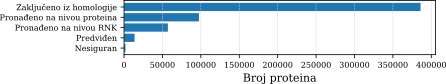
\includegraphics[]{plots/PE.pdf}
  \label{fig:PE}
  \caption{Histogram nivoa pouzdanosti \swissprot proteina}
\end{figure}

% \section{Disprot}
%
% Baza proteinskog neuređenja \en{Database of protein Disorder (DisProt)}
%
% \section{D2P2 i MobiDB}
%
% Baze predviđenog neuređenja proteinskih sekvenci















\chapter{Podaci i Metode} % Main chapter title

\label{Podaci i Metode} % For referencing 



\section {Podaci}

Za metode koje prezentujemo potrebne su tri vrste informacija:
\begin{enumerate}
  \item Što više različitih proteina.
  \item Pouzdana anotacija funkcija.
  \item Informacije o funkcijama, prvenstveno međurelacije.
\end{enumerate}

Međurelacije između funkcija su bitne samo ako je potrebno grupisati ih,
ili ako je potrebno mapiranje na neku drugu nomenkulaturu funkcija pa
se zahteva grupisanje.


\subsection{Podaci iz originalnog rada}

U originalnom radu \parencite{Xie2007} korišćena je  baza ručno proverenih
proteinskih sekvenci \keyword{Svis-Prot} \en{Swiss-Prot}, verzija 48 iz 2005.
Verzija 48 ima 201 560 proteina od kojih 196 326 imaju dužinu preko 40
aminokiselina (što je potrebno zbog definicije ref \ref{pdis_def}). Funkcije
pridružene proteinima izražene su \keyword{kontrolisanim vokabularom}
\en{controlled vocabulary} koga čine takozvane UniProtKB \keyword{ključne reči}
\en{keywords}. U verziji 48, UniProtKB sadrži 874 ključnih reči.  Zbog
statističke značajnost posmatrane su one ključne reči kojima je bilo anotirano
barem 20 proteina, tj. 710 ključnih reči.

Proteinske sekvence u Svis-Prot bazi ''nisu redundantne'' u smislu da 
su produkti jednog gena za jednu vrstu predstavljeni jednim entiteom 
\parencite{nonRedundant}. Zbog toga unosi u bazu tretiraju se kao proteini a ne
pojedinačne proteinske sekvence.
Međutim za analizu funkcija podaci su \keyword{statistički redundantni} jer
sadrže jako mnogo \keyword{homologih} proteina. Rešenje  klasterovati proteine
u \keyword{proteinske familije}, čime je dobijeno 27 217 familija.  Tada svaki
protein ima težinu kojom doprinosi analizi funkcija tako da je težina svih
proteina jedne familije uniformno raspoređena i sabira se na jedan.  Za detalje
konsultovati originalni rad. \parencite{Xie2007}.

\textbf{komentar:} \\
Ono što autori nisu elaborirali jeste da početni uslov od minimum 20 proteina
po ključnoj reči možda nije dovoljan. Ako pretpostavimo zarad ilustracije
normalnu raspodelu veličina klastera proteina, očekivali bi da klaster najčešće
sadrži 7 proteina. Dakle iako je 50 proteina pridruženo nekoj funkciji ona
verovatno ima pridruženih svega 7 familija proteina. Kako familija sadrži
proteine pod pretpostavkom istog evolutivnog porekla njihova funkcija bi
trebalo da je slična pa se onda postavlja pitanje da li je 7 familija dovoljno
da bi se razmatrala data ključna reč. Ovo je primarno kritika za ključne reči
jer one obično predstavljaju jako opšte pojmove.

Sa druge strane za usko specijalizovane pojmove bila bi dovoljna jedna familija
proteina jer bi ona predstavljala sve razne homologe (TODO Burkhard Rost,
Termofili)



\subsection{Naši podaci (CAFA3 proteini)}

U ovom radu korišćen je skup proteina preuzet sa \keyword{CAFA3} takmičenja gde
je korišćen kao trening skup za predikciju funkcija proteina \parencite{CAFA}.
Podaci se sastoje od dve datoteke:

\begin{enumerate}
  \item \file{uniprot\_sprot\_exp.fasta}  sadrži 41 793 proteina od kojih
         41 227 ima dužinu veću od 40 aminokiselina.
  \item \file{uniprot\_sprot\_exp.txt} pridružuje funkcije označene kao
        \keyword{GO termini} \en{Gene Ontology terms}. Postoje
        termini iz sve tri ontologije: 16 117 ćeliskih komponenti,
        5 966 molekulskih funkcija i 16 117 bioloških procesa.Jednom proteinu
        može biti pridruženo više GO termina i obrnuto.
\end{enumerate}

CAFA3 trening skup je pažljivo odabran podskp Swis-Prot proteina i smatra se da
nije \keyword{statistički redundantan} \parencite{??}. Iz tog razloga nije
potrebno vršiti klasterovanje i analiza je jednostavnija te u metodama
predstavljamo samo jednostavan oblik formula koje odgovaraju CAFA3 podacima.

Sekvence su kodirane jednim karakterom i koristeći \keyword{IUPAC} kodove.
Među proteinima bilo je sekvenci sa nestandardnim aminokiselinam 'U'
i 'O' ili višeznačnim oznakama 'B', 'J', 'X' i 'Z'. Ovi proteini se preskočeni jer
ih VSL2b predkitor ne podržava. Nakon filtiranja ostalo je 41 119 proteina.

U ovom radu analiziraćemo samo termine molekulskih funkcija.  Od 5 966 termina
svega 358 ima pridruženo 20 ili više proteina. Zbog prirode ontologija ovaj broj
se može povećati uopštavanjem termina sa malim brojem pridruženih proteina ili
obrnuto specijalizacijom onih sa velikim brojem pridruživanja. Detaljan postupak
uopštavanja i specijalizacije objašnjen je u metodama.


\section {Metod}

Cilj rada bio je ispitivanje veze između molekulske funkcije proteina i njegove
(ne)uređenosti tj.  da li ona zavisi više od uređenosti ili neuređenosti.

\textbf{Idealan slučaj.} 
Pretpostavimo da za proizvoljnu molekulsku funkciju imamo skup različitih
proteina.  Da bi dali korektan odgovor na ovo pitanje moramo da znamo kako
neuređenost pojedinačnog proteina utiče na zadatu funkciju, da li je bitna ili
nije bitna. Nije dovoljno samo posmatrati da li protein ima neuređeni region
jer možda on ne utiče na funkciju. Ovaj pristup zahteva ekspertsko poznavanje
svakog proteina i anotirane funkcije te stoga  može da se primeni na jako malo
funkcija. Takođe, trenutno svega 803 proteina ima eksperimentalno opisanu
neuređenost \parencite{disprot} 

\textbf{Realnost.} 
Možemo da damo procenu ako pretpostavimo da veći udeo neuređenih u odnosu na
uređene proteine podrazumeva da funkcija zavisi više od neuređenosti.  Dakle
ono što želimo jeste da ispitamo \keyword{korelaciju} između funkcije i
(ne)uređenosti proteina kojima je pridružena. Ali prvo potrebno je definisati
šta znači da je protein neuređen. Definicija mora da ima biološkog smisla za
analizu ali pored toga je ograničena je sposobnostima i preciznošću prediktora
koji se korist. Više o tome u nastavku.


\subsection{Predikcija dugih neuređenih regiona}

Autori \parencite{Xie2017} koristili su \keyword{PONDR VL3E} prediktor koji
postiže tačnost od $~87\%$ pri unakrsnoj validaciji nad uravnoteženim test
skupom.  Zbog ekonomičnosti i dostupnosti mi smo koristili \keyword{PONDR
VSL2b}.

Oba prediktora pripadaju \keyword{PONDR} \en{(Predictor Of Naturally Disordered
Regions)} familiji prediktora. Ovi prediktori zasnivaju se na eksperimentalno
pokazanim karakteristikama neurđenih regiona. Preciznije određene aminokiseline
verovatnije su da se jave u neuređenom regionu. Neuređeni regioni imaju manje
aromatičnih i hidrofobnih AK, veći ukupni naboj, veći indeks fleksibilnost i
manju kompleksnost sekvence. Ove osobine izražene kao atributi koriste se za
treniranje neuronske mreže \en{neural networks} sa propagacijom unapred \en
{feed forward} koja koristi prozor veličine između 9 i 21 aminokiseline.
Finalni prediktor predstavlja kombinaciju nekoliko neuronskih mreža gde je
svaka od njih trenirana nad različitim podacima specijalizujući se da predviđa
samo regione određene veličine ili položaja. PONDR familija ima nekoliko
prediktora koji  se razlikuju u načinu treniranja što se postiže kombinacijom
različitih trening skupova.  Oznaka ''VSL2b'' kodira tipove proteinskih skupova
nad kojima su trenirani prediktori.
\begin{itemize}
  \item V - Opisuje eksperimentalnu tehniku kojom je neurđenost utvrđena na
    trening skupu \en{X-ray, NMR, circular dichroism}
  \item S - Prediktor je treniran na skupu proteina sa \keyword{kratkim}
      neruređenim
    regionim ($<30$ AK)
  \item L - Prediktor je treniran na skupu proteina sa \keyword{dugim}
    neuređenim regionima ($>30$ AK)
\end{itemize}

VSL2b kao ulaz prima proteinsku sekvencu minimalne dužine 9 AK kodiranih jednim
karakterom. Podržava azbuku od samo 20 standardnih AK.  Izlaz je niz
ocena(verovatnoća) za svaku aminokiselinu da li pripada neuređenom regionu to
jest da je taj rezidual
\footnote{ Rezidual je čest naziv koji se koristi za elemente na nekoj
  poziciji sekvence.  Koristi se za aminokiseline  proteina ali i za nukleinske
  kiseline kod DNK i RNK.  Naziv potiče od hemiskih tehnika prečišćavanja čiji
  su rezultati reziduali (ostaci).
} neuređen. Reziduale sa vrednošću iznad 0.5 smatramo neuređenim a suprotno
uređenim. Za potrebe analize autori uvode sledeću definiciju:\\

\newtheorem{mydef}{Definicija}
\begin{mydef}
\label{pdis_def}
Protein je \keyword{verovatno/putativno neuređen} \en {putatively disordered} ako
sadrži bar jedan region veći ili jednak od 40 uzastopnih aminokiselina
takvih da imaju \textit{predviđenu neuređenost} iznad 0.5. \\
\end{mydef}

Onda definišemo operator $d$ takav da za svaku proteinsku sekvencu $s_i$ važi:


\[   
  d(s_i) = 
    \begin{cases}
      1 & \text{ako je} \quad s_i \quad \keyword{verovatno neuređena}\\
      0 & \text{suprotno}
    \end{cases}
\]


\subsection{Zavisnost dužine proteina i predikcije dugačkog neuređenog regiona}

Verovatnoća da po gornjoj definiciji protein bude klasifikovan kao verovatno
neuređen raste sa porastom njegove dužine. Ovo je ozbiljan problem koji utiče
na statističku značajnost rezultata. Autori \parencite{Xie2007} predstavljaju način
da se ta verovatnoću proceni.
Označimo tu verovatnoću sa $P_L$ gde $L \in N$ označava dužinu sekvence. Neka
je $V_L$ skup svih validnih proteina dužine $L$ onda bismo $P_L$ mogli da
procenimo kao količnik broja verovatno neuređenih proteina iz $V_L$ i ukupnog
broja proteina u $V_L$. Ovaj idealan slučaj nije realan jer skup svih
validnih proteina nije poznat. Pod validnošću podrazumevamo da se protein
javlja prirodno kao produkt evolucije (tj. ima ili je imao funkciju u
organizmu). Skup $V_L$ aproksimiraćemo  skupom svih naših proteina. Međutim,
ovaj skup je suviše mali i $P_L$ sadrži mnogo šuma. Da bi uglačali rezultat
autori \cite{Xie2007} predlažu da se umesto skupa proteina egzaktne dužine $L$
koristi skup  proteina u oznaci $S_L$ sa dužinama između $[L-l, L+l]$ gde je $l
= 0.1*L$. Dobijamo sledeće formule:

$$ S_L = \{s_i \mid \quad | L -  \Vert s_i \Vert | <= l \quad   \}$$
$$ P_L = \dfrac{ \sum_{s_i \in S_L} d(s_i)} {\Vert S_L \Vert}$$

Ponašanje $P_L$ predstavljeno je na grafiku \ref{fig:PL1}. Glatkoća rezulatata
kontroliše se veličinom $l$ koja predstavlja prozor uprosečavanja. Kako je $l =
0.1*L$ tako da prozor uprosečavanja raste sa porastom dužine proteina te $P_L$
postaje glađe sa veličinom proteina. Za konstantni prozor uprosečavanja ova
tehnika je još poznata kao \en{rolling average} ili \en{boxcar filter} i
pripada specijalnoj vrsti konvolucije. Trenutno ne znamo zašto se autor odlučio
da veličina prozora raste sa dužinom proteina.


\begin{figure}[th]
\centering
\includegraphics[]{../plots/PL_F}
\decoRule
\caption {
 Punom linijom predstavljena je $P_L$ sa prozorom uprosečavanja $l = 0.1L$,
 a krstići predstavljaju sirove vrednosti $l = 0$ 
}
\label{fig:PL1}
\end{figure}


Pored gore prikazanog 'originalnog' metoda predstavljamo još jedan pristup.
\keyword{Slučajno generisani} \en{random generated} proteini za procenu $P_L$.
Razmotrićemo dva modela. Prvi je naivan model \keyword{uniformne verovatnoće}
koji podrazumeva da se svaka aminokiselina javlja sa istom verovatnoćom odnosno
$1/20$. U statistici ovo je još poznato kao \en{equiprobable model}.  Drugi
model koji ćemo zvati 'slučajni' ili 'random' model predstavlja slučajnu
promenljivu čija verovatnoća zavisi od učestalosti aminokiselina iz CAFA3 skupa
i prikazana je na grafiku \ref{fig:ucestalost_AK}.  Koristeći ova dva modela za
svaki protein generisan je slučajan protein iste dužine koji se koristi za
procenu $P_L$.


\begin{figure}[th]
\centering
% \includegraphics[scale=0.7]{Figures/ucestalost_AK}
\includegraphics[]{../plots/ucestalost_AK}
\decoRule
\caption{Učestalost aminokiselina u podacima}
\label{fig:ucestalost_AK}
\end{figure}



Poređenje ova dva pristupa sa originalnim $P_L$ prikazano je na slici
\ref{fig:PL2}.  Originalni $P_L$ ostaje prikazan kao puna linija. Jasno se vidi
da slučajni model prikazan isprekidanom linijom predstavlja vizuelno dobru
aproksimaciju dok uniformni model verovatnoća prikazan tačkicama znatno odstupa
i dosta sporije raste (reklo bi se skoro linearno). Kako VSL2b predkitor
prepoznaje neuređene regione na osnovu učestalosti aminokiselina ovo ponašanje
nije čudno jer je manja verovatnoća pojave aminokiselina koje promovišu
neuređenost. Zbog suviše velikog odstupanja uniformni model nije korišćen u
daljoj analizi.


\begin{figure}[th]
\centering
% \includegraphics[scale=0.65]{Figures/PL2}
\includegraphics[]{../plots/PL_F_cmp}
\decoRule
\caption{Različiti pristupi za procenu $P_L$}
\label{fig:PL2}
\end{figure}


Jedno objašnjenje zašto je uniformni model naivan i toliko odstupa od
prvobitnog metoda proizilazi iz činjenice da aminokiseline imaju inherentno
različite verovatnoće. Naime  aminokiseline ne mogu  imati istu
verovatnoću jer se  broj njihovih kodona razlikuje. Neke aminokiseline
su kodirane sa samo jednim a druge i sa 6 kodona. Očekivali bi da broj kodona
povećava učestalost aminokiseline i ta korelacija uz izuzetke arginina se vidi
na slici
\ref{fig:aminoacid} \parencite{AKfrekvencija}.

\begin{figure}[th]
\centering
\includegraphics[scale=0.7]{Figures/aminoacid}
\decoRule
\caption{očekivana i realna učestalost  aminokiselina kod sisara}
\label{fig:aminoacid}
\end{figure}



\subsection{Ocenjivanje zavisnosti funkcije od neuređenosti}

Neka je $S_j$ skup proteina koji imaj pridruženu funkciju $j$. Tada procenat
verovatno neuređenih proteina $F_j$ možemo izračunati kao: $$F_j =
\dfrac{\sum_{s_i \in S_j} d(s_i)} {\Vert S_j \Vert} $$

Nultu hiptezu koja predviđa da je rezultat $F_j$ posledica samo slučajnosti to
jest zavisi samo od $P_L$ opisaćemo preko slučajne veličinu $Y_j$.  $$ Y_j =
\dfrac {\sum_{s_i \in S_j} {X_{|s_j|}}}{\Vert S_j \Vert}$$ Gde je $X_L$
Bernulijeva slučajna veličina sa verovatnoćom $P(X_L = 0) = P_L$ odnosno $P(X_L
= 1) = 1-P_L$

Ako $F_j$ izlazi iz intervala poverenja raspodele $Y_j$ onda funkcija $j$
sadrži značajno mnogo predviđenih neuređenih ili uređenih proteina. Preciznije
ako je \textit{p-value} $<0.05$ funkcija $j$ je povezana sa neuređenim
proteinima a ako je \textit{p-value} $>0.95$ funkcija $j$ je povezana sa
uređenim proteinima. Suprotno ne možemo ništa da tvrdimo za funkciju $j$.

$Y_j$ je teško izračunati analitički tako da se pribegava empiriskom
računanju p-vrednosti. Empiriska p-vrednost se određuje tako što se za 1000
realizacija gleda frakcija koliko puta je realizovano  $Y_j$ bilo veće od
$F_j$.
Za veće skupove $S_j$ raspodela $Y_j$ liči na normalnu pa računanjem očekivanja
$\mu_j$ i standardne devijacije $\delta_j$ za raspodelu $Y_j$ možemo da
izračunamo Z-skor kao $Z_j=(F_j-\mu_j)/\delta_j$. Dalje p-vrednost možemo da
aproksimiramo kao $1/2(1-erf(Z_j/2)))$ ako raspodela liči na normalnu.  Ovo je
nekad korisno jer sa 1000 realizacija $Y_j$ nemamo dovoljnu preciznost da
računamo p-vrednost veću ili manju od 0.01 i 0.99. Ipak koristićemo samo
empiriski izračunatu p vrednost.

\section {uopštavanje, grupisanje  GO termina}

\section {Metod za upoređivanje rezultata}


\chapter{Priprema podataka} % Main chapter title

\label{Priprema_podataka} % For referencing 

\section{Objedinjavanje CAFA3-skupa i baze \swissprot}
\label{objedinjavanje}

Povezivanje proteina iz CAFA3-skupa sa slogovima iz baze \swissprot je jedini
način da se dođe do anotacija ključnim rečima. Takođe, ovim procesom dobili smo
najnovije anotacije GO-termina ali i dodatne informacije, na primer taksonomsko
poreklo proteina koje pomaže u razumevanju skupa podataka.

Iz CAFA3-skupa izdvojeni su svi validni proteini (dužine barem 9 i azbuke od 20
standardnih aminokiselina). U ovom koraku ne izbacujemo proteine kraće od 40
AK.  Sadržaj baze \swissprot preuzet je iz datoteke
\file{uniprot\_sprot-only2017\_12} \cite{sprot} koja sadrži 556 196 proteina.
Od 66 599 validnih proteina iz CAFA3-skupa 66 530 ima nepromenjen primarni
identifikacioni broj (AC), dok 69 slogova iz baze \swissprot sadrže nedostajuće
primarne AC kao sekundarne. Kao što je navedeno u Potpoglavlju \ref{svis-prot}
ovo je posledica dva moguća mehanizma:

\begin{enumerate}
  \item Specijalizacija jednog proteina iz CAFA3-skupa u više različitih
    slogova.  Zbog moguće statističke redundantnosti ovi slogovi su zanemareni.

  \item Unifikacija nekoliko proteina iz CAFA3-skupa pod novi slog.

  \begin{figure}[th]
  \centering
  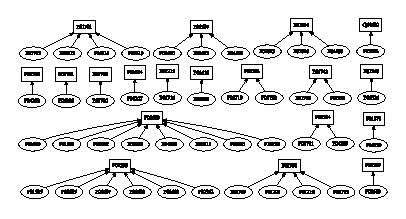
\includegraphics[scale=2]{plots/unifikacija_slogova2.eps}
  \caption{Unifikacija starih (elipse) sa novim slogovima iz baze \swissprot}
  \label{fig:unifikacija_slogova}
  \end{figure}

\end{enumerate}

Rezultat unifikacije prikazan je na Slici \ref{fig:unifikacija_slogova}.
Međutim, analizom ovih promena uspešno su rekonstruisana svega četiri nova sloga
koja odgovaraju nedostajućim proteinima. Kako je četiri suviše malo, zbog
jednostavnosti ih nismo ubrajali u dalju analizu te koristimo samo 66 530
slogova čiji su primarni identifikatori nepromenjeni.


Validini proteini iz CAFA3-skupa anotirani su sa  5 957 različitih GO-termina
molekulske funkcije (MF) od kojih je 50 zastarelo i izbačeno iz \file{go.obo}
datoteke.  Za bazu \swissprot nismo bili u mogućnosti da proverimo samo MF,
ali ukupno je izbačeno 319 GO-termina.  CAFA3-skup sadrži 67 MF koje se ne
javljaju u anotacijama iz baze \swissprot dok baza \swissprot sadrži 888 MF
koje se ne javljaju u anotacijama CAFA3-skupa.  Pošto je korišćena verzija baze
\swissprot novijeg datuma, anotacija iz CAFA3-skupa su zanemarene u korist
novijih anotacija iz baze \swissprot. Ove razlike sumirane su  Tabelom
\ref{tab:godiff}

\begin{table}[htpb]
\begin{tabular}{|r|c|c|}
  \hline
                  & CAFA3 & \swissprot \\
  \hline
  MF-termini      & 5 957 &    7 471    \\
  nedostaje u go.obo   & 60 MF & 319 MF, CC i BP \\
  MF, samo u:   & 67    & 888             \\
  \hline
\end{tabular}
  \centering
  \caption{Razlike u GO-terminima između CAFA3-skupa i baze \swissprot}
  \label{tab:godiff}
\end{table}

Dodatno, baza \swissprot sadrži 194 proteina čije se sekvence razlikuju u
odnosu na proteine iz CAFA3-skupa. Odlučili smo da zadržimo originalne proteine
iz CAFA3-skupa.

\section{Grupisanje proteina po GO-terminima}
\label{grupisanje}

Kao što je bilo reči u Sekciji \ref{ocenjivanje} sa $S_A$ označavamo skup
proteina koji obavljaju funkciju $A$, odnosno funkcija $A$ anotira proteine
grupisane skupom $S_A$.  Ako je GO-termin $A$ potomak GO-termina $B$ tj. važi
$A$ \textit{is\_a} $B$ i želimo da diskutujemo o funkciji $B$, onda i svi
proteini anotirani funkcijom $A$ (i time pripadaju skupu $S_A$) treba da budu
sadržani i u skupu $S_B$.  Primetili smo da anotacije ključnih reči već
podrazumevaju opisano grupisanje.  Na primer, ključna reč
\textit{Ribosomalprotein} anotira 1420 proteina, a njen predak (uopštenje)
\textit{Ribonucleoprotein} takođe anotira pomenutih 1420 proteina, plus
dodatnih 478 proteina.  Anotacije GO-terminima ne podrazumevaju ovakvo
grupisanje u eksplicitnom smislu.  Preciznije, zbog granularnosti ontologije
bilo bi suviše redundantno ponavljati antoacije za svakog pretka GO-termina.
Primer se može videti na Slici \ref{fig:neuropeptide} iz Potpoglavlja
\ref{kw2go_mapiranje}.
 
Za implementaciju predloženog grupisanja koristili smo algoritam topološkog
sortiranja. Ovako formirani skupovi koji sadrže manje od 20 proteina nisu bili
od značaja za dalju analize zbog čega su odbačeni.
Ovom metodom dobijen je 1781\footnote{Bez ovog grupisanja imali bismo samo 1146
MF-termina  koji zadovoljavaju uslov od najmanje 20 proteina.} MF-termin (od ukupno
11 135 validnih MF-termina) sa po najmanje 20 pridruženih proteina uključujući i
koreni\footnote{Koreni termin ili koreni čvor ontologije tj.  termin
\textit{molecular function}.} termin. U ovom koraku uračunati su samo proteini
minimalne dužine 40 AK.

% \section{Ontologije gena i ključne reči}
\section{Preslikavanje između GO-termina i ključnih reči}
\label{kw2go_mapiranje}

Kako je ovo istraživanje ograničeno na molekulske funkcije, u daljem tekstu
biće razmatrana preslikavanja isključivo između ključnih reči kategorije MF koje
zovemo \keyword{ključne reči MF} i GO-termina iz imenskog prostora MF koje zovemo
\keyword{MF-termini}. Pokazaćemo da ovo nije trivijalan zadatak i da u opštem
slučaju zbog razlika u nomenklaturi preslikavanje ne postoji ili da pronađene
funkcije nisu uvek ekvivalentne.

U referentnom radu navodi se da je baza \swissprot sadržala 143 ključne reči MF
dok  datoteka \file{keywlist.txt} \cite{keywlist_txt} iz 20.12.2017 sadrži 195.
Nažalost, nismo pronašli  \file{keywlist.txt} datoteku iz 2006. godine pa ne
znamo egzaktnu razliku, ali jasno je da su neke ključne reči
izbačene ili zamenjene a neke samo dodate. Datoteka \file{keywlist.txt} opisuje
ključne reči, a sadrži i pridruživanja (relaciju) odgovarajućim GO-terminima.
Pomenuta relacija pridružuje ključne reči MF ne samo MF-terminima već i
GO-terminima imenskih prostora BP i CC . Strogo posmatrano pridruživanja ne
čine funkciju (preslikavanje), jer se neke ključne reči MF pridružuju većem
broju GO-termina čak i ako ograničimo sliku preslikavanja na samo
MF\footnote{Samo \textit{DNA invertase} se preslikava u dva različita
MF-termina (\textit{DNA binding} i \textit{recombinase activity}).} ili samo
BP-termine.  Ipak, opisana pridruživanja nazivaćemo preslikavanja ili direktna
preslikavanja. Direktna preslikavanja za ključne reči MF sumirana su Tabelom
\ref{tab:direktna_map}.  Za 20 ključnih reči MF uopšte ne postoji preslikavanje
dok je broj preslikavanja ka MF, BP i CC imenskim prostorima, redom 104, 54 i
11. Dakle, veliki broj preslikavanja ka MF-terminima nedostaje.

\begin{table}[htpb]
\begin{tabular}{|r|c|c|c|c|c|}
  \hline
                   & ukupno & nema pres. & pres. MF & pres. BP & pres. CC.      \\
  \hline
   ključne reči MF & 195    &  20       &  104     & 54      & 11           \\
  \hline
\end{tabular}
  \centering
  \caption{Direktna preslikavanja za ključne reči MF}
  \label{tab:direktna_map}
\end{table}

Nedostajuća preslikavanja ka MF-terminima pogotovo dolaze do izražaja kod
neuređenih ključnih reči MF (Definicija \ref{neuredjena_funkcija}) .Slika
\ref{fig:KWtop20dis} prikazuje direktna preslikavanja za 20 statistički
najznačajnijih (Definicija \ref{stat_naj}) neuređenih ključnih  reči MF
preuzetih iz referentnog rada \parencite{Xie2007}.  Tri ključne reči MF nemaju
direktno preslikavanje, dve se preslikavaju na ćelijske komponente, osam na
biološke procese i svega šest na molekulske funkcije dok ključna reč MF
\textit{Antigen} više ne postojii. Sa druge strane, od 20 statistički
najznačajnijih uređenih ključnih reči MF iz referentnog rada samo jednoj fali
direktno preslikavanje.

\begin{figure}[!th]
\centering
\hspace*{-1.5cm} 
\includegraphics[scale=0.9]{Figures/plots/kw_dis2go.pdf}
\caption {
  Direktno preslikavanje 20 statistički najznačajnijih neuređenih ključnih reči MF
  \parencite{Xie2007} na GO-termine.  Statistički najznačajne ključne reči MF su
  ljubičaste dok radi kompletnosti navodimo neke njihove specijalizacije i
  generalizacije koje su obojene sivo. GO-termini su predstavljeni manjim
  kružićima.
}
\label{fig:KWtop20dis}
\end{figure}

Nedostajuća preslikavanja ka MF-terminima (skoro polovina ključnih reči MF) ne
samo da otežavaju poređenje pojedinačnih ključnih reči već predstavljaju
metodološki problem za poređenje nomenklatura.  Referentni rezultati su uređeni
prema statističkoj značajnosti (Z-skor za $F_j$) i predstavljaju dve tabele od
20 statistički najznačajnijih neuređenih odnosno 20 uređenih ključnih reči MF
(zanemarujući roditeljski odnos između njih). Na nivou ključnih reči ovo nije
problem, ali ako bi se isti postupak primenio na MF-termine poredili bi manje
od 200 ključnih reči MF sa potencijalno preko 11 000 MF-termina. Potrebno je
odabrati dovoljno opšte MF-termine, takve da čine reprezentativan uzorak
molekulskih funkcija i da njihovo sortiranje po Z-skoru (kao u referentnom
radu) ima smisla.  Biće predložena dva pristupa za automatsko biranje opisanih
MF-termina dok je ručni odabir izvan obima ovoga rada.  Oba pristupa imaju
sličnu ideju koja podrazumeva izdvajanje samo onih MF-termina koji su
pridruženi ključnim rečima MF.  Međutim, kako polovina preslikavanja nedostaju
(Tabela \ref{tab:direktna_map}), neophodno je dopuniti nedostajuća
preslikavanja zarad smislenosti poređenja.  Automatski metodi koje ćemo
predložiti razlikuju se u načinu pronalaženja ovih nedostajućih preslikavanja.
Treba primetiti da, čak i da nema nedostajućih preslikavanja, ovaj pristup
zanemaruje statistički značajne MF-termine koji nemaju ekvivalentne ključne
reči MF. 



\clearpage

\subsection{Metod indirektnih preslikavanja}

Rezonujući nad relacijama ontologije gena, moguće je doći do
\keyword{indirektnih preslikavanja} koja preko BP ili CC termina vode ka
MF-terminima. Neki MF-termini su relacijama \keyword{part\_of} i
\keyword{has\_part} povezani sa BP ili CC terminima, mada postoje MF-termini
koji nikako nisu povezani sa terminima ostalih  ontologija. Traženje
indirektnih preslikavanja izvršeno je korišćenjem \keyword{Neo4j} grafovkse
baze.  Za sve ljubičaste BP-termine sa Slike \ref{fig:KWtop20dis} i sve njihove
specijalizacije provereno je da li su nekom (bilo kojom) relacijom u vezi sa
nekim (bilo kojim) MF-terminom. Pronađeno je samo jedno indirektno
preslikavanje, zajedničko za ključne reči MF \textit{Neuropeptide} i
\textit{Endorphin}. Za tri pomenuta CC termina indirektna preslikavanja nisu
pronađena. 


Razmotrimo pronađeno preslikavanje za ključnu reč MF \textit{Neuropeptide} i
proteine koji su anotirani razmatranim MF-terminima. Slika \ref{fig:neuropeptide}
generisana je \keyword{Cypher}\footnote{\textit{Cypher} je upitni jezik za
Neo4j grafovsku bazu.} upitom koji koji pored GO-termina takođe vraća anotirane
proteine. Preciznije, upit prvo pronalazi direktno preslikavanja (BP-termin)  a
zatim sve potomke (indirektne MF-termine) i na kraju anotirane proteine.
Proteini su preuzeti iz CAFA3-skupa. 

{ \fontsize{9}{9} 
\begin{verbatim}
MATCH p=(:Keyword {name:"Neuropeptide"})--(:GOTerm)<-[*0..]-(:GOTerm)<--(:Prot)
RETURN p
\end{verbatim}
}

\begin{figure}[!th]
\centering
% \hspace*{-1.0cm} 
\includegraphics[scale=0.677]{Figures/plots/Neuropeptide2go.pdf}
\caption {
  Preslikavanje ključne reči MF \keyword{Neuropeptide} na MF-termin
  \textit{Neuropeptide receptor activity} preko relacije \keyword{part\_of}.
  Dobijeno preslikavanje rezultuje malim brojem zajednički anotiranih proteina.
}
\label{fig:neuropeptide}
\end{figure}

Sa Slike \ref{fig:neuropeptide} jasno se uočava da ključna reč MF
\textit{Neuropeptide} deli svega 5 anotacija sa svim pronađenim MF-terminima.
Smatramo da je zbog male sličnosti u anotacijama pronađeno indirektno
preslikavanje nevalidno, jer se očigledno ključna reč MF \textit{Neuropeptide} i
MF-termin \textit{Neuropeptide receptor activity} koriste u različitim
kontekstima. Zapravo, šablonski naziv pronađenog MF-termina (po pravilima iz
Potpoglavlja \ref{MF}) označava da se termin koristi za anotiranje proteina
koji se \textit{vezuju za neuropeptid zarad inicijacije neke ćelijske
funkcije}, a ne samih neuropeptida. Takođe, treba primetiti da je pronađeni MF-termin povezan na BP-termin relacijom \keyword{part\_of}.  Ovo može da
predstavlja još jedan razlog zašto je pronađeno preslikavanje nevalidno.  Veza
\keyword{part\_of} podrazumeva agregaciju a ne kompoziciju. Agregacija
podrazumeva da  molekulska funkcija postoji nezavisno od biološkog procesa što
je suprotno od kompozicije koja predstavlja relaciju \keyword{has}. Nažalost,
nijedan od osam pomenutih BP-termina nema relaciju \keyword{has} ka nekom MF-terminu.

\clearpage

Kao što je bilo reči u Potpoglavlju \ref{MF}, molekulske funkcije ne mogu da
predstavljaju gene ili genske produkte već funkcije koje oni obavljaju. Ključna
reč \keyword{Neuropeptide} po definiciji predstavlja peptide koje neuronske
ćelije oslobađaju ili hormone koji se oslobađaju iz drugih tipova ćelije. Jasno
je da ekvivalentan MF-termin ne može da postoji.  Nažalost, postoji veliki broj
ključnih reči MF koje iz ovog razloga ne mogu da imaju ekvivalentan MF-termin,
na primer: \textit{ Neurotoxin, Endorphin, Pyrogen, Milk protein, GAP protein,
Motor protein, Myosin, ...}. Veliki broj ovakvih ključnih reči MF objašnjava 
zašto skoro pola direktnih preslikavanja na MF-termine ne postoji.  Zbog svih
navedenih problema, zaključili smo da indirektna preslikavanja nisu adekvatna za
primene u ovom radu.

Ipak, treba pretpostaviti da je za neke ključne reči moguće pronaći MF-termin
koji predstavlja zajedničku molekulsku funkciju za skup proteina anotiran
polaznom ključnom reči MF.  U cilju pronalaženja takvih MF-termina u nastavku
predlažemo jednostavan metod zasnovan na sličnosti skupova.

\subsection{Metod sličnih anotacija}

\keyword{Metod sličnih anotacija} pretpostavlja da dve ekvivalentne funkcije (iz dve
različite nomenklature) anotiraju sličan skup proteina.  Jedan način da se
definiše sličnost između dva skupa $A$ i $B$ je preko \keyword{Žakardovog indeksa}
\en{Jaccard index}, kraće \keyword{Ji}  definisanog sledećom formulom:
$$J(A,B) = \dfrac{|A \cap B|}{|A \cup B|} =  \dfrac{|A \cap B|}{|A|+|B|-|A \cap B|}$$
$$  J(A,B) \in [0, 1] $$
\[   
  J(A,B) = 
    \begin{cases}
      1,&A=B  \\
      0,&A\cap B=0
    \end{cases}
\]
Za realizaciju ove metode korišćeni su svi proteini iz baze \swissprot, ne samo iz
CAFA3-podskup.  Neka skup $A$ predstavlja proteine koje anotira ključna reč MF $kw_A$
a skup $B$ proteine koje anotira MF-termin $t_B$.  Zbog jednostavnosti računske
metode, skup B nije dobijen grupisanjem opisanim u Potpoglavlju
\ref{grupisanje}, dakle ne sadrži proteine specifične za potomke termina $t_B$
već samo sirove anotacije iz baze \swissprot.  Za $kw_A$ najverovatnije
preslikavanje predstavlja MF-termin $t_B$, takav da je Žakardov indeks $J(A,B)$
najveći.  Ipak, ne treba očekivati da će najveći Žakardov indeks nužno značiti
i najpogodnije preslikavanje. Iz tog razloga potrebno je  sagledavati nekoliko
najboljih predloga za preslikavanje, sortiranih opadajuće po veličini
Žakardovog indeksa. Preslikavanja dobijena ovim postupkom zvaćemo
\keyword{izvedena preslikavanja}.

Pouzdanost predloženog metoda testirana je nad 104 ključne reči MF sa poznatim
direktnim preslikavanjem.  Za svaku ključnu reč izdvojili smo maksimum pet
najverovatnijih izvedenih preslikavanja. Izvedna preslikavanja sa najvećim Žakardovim
indeksom poklapaju se sa poznatim direktnim preslikavanja za 61 ključnu reč
($59\%$). Razmatranjem izvedenih preslikavanja nižeg Žakardovog indeksa moguće
je povećati broj korektnih preslikavanja na 90 ($85\%$).

Opisani metod uz razmatranje maksimum 5 najpogodnijih izvedenih preslikavanja
primenili smo nad 91 ključnu reč MF sa nedostajućim direktnim preslikavanjem.
Izvedena preslikavanja sa Žakardovim indeksom manjim od 0.1 nisu razmatrana što
je automatski eliminisalo 25 ključnih reči MF iz daljeg razmatranja. Nakon
ručnog pregledanja dobijena su 64 izvedena preslikavanja. Zbog domena problema,
ne možemo da tvrdimo da su pronađena preslikavanja korektna. Pogotovo su
problematična preslikavanja sa niskim Žakardovim indeksom (ispod 0.3). Ipak,
treba uzeti u obzir da niži Žakardov indeks može biti posledica izostanaka
grupisanja (Potpoglavlje \ref{grupisanje}) proteina po MF-terminima.

Tabela \ref{tab:izvedeno_mapiranje} prikazuje izvedena preslikavanja sa
minimalnim Žakardovim indeksom 0.2 izuzev poslednja tri reda. Poslednja tri
reda i ostali redovi sa zadebljanim tekstom \en{bold text} predstavljaju
nedostajuća direktna preslikavanja sa Slike \ref{fig:KWtop20dis}.


\begin{table}[htpb]
  \centering
  % \hspace*{-2.0cm} 
  \footnotesize
  \begin{tabular}{|p{4.7cm}|c|c|c|p{5cm}|}
  \hline
  \bf \textit{ključna reč MF} & \bf n\_kw & \bf Ji & \bf n\_go & \bf \textit{MF-termin} \\
  \hline
  \hline
  Dermonecrotic toxin                & 148   & 0.96  & 142   & phospholipase D activity \\ \hline
  \keyword{Ribosomal protein}        & 49054 & 0.91  & 48096 & structural constituent of ribosome \\ \hline
  Complement system impairing  toxin & 160   & 0.81  & 142   & phospholipase D activity \\ \hline
  Hemagglutinin                      & 397   & 0.75  & 299   & host cell surface receptor binding \\ \hline
  Mutator protein                    & 255   & 0.75  & 288   & damaged DNA binding \\ \hline
  Antifreeze protein                 & 10    & 0.7   & 7     & ice binding \\ \hline
  Light-harvesting polypeptide       & 90    & 0.68  & 61    & bacteriochlorophyll binding \\ \hline
  Cyclin                             & 197   & 0.61  & 124   & cyclin-dependent protein serine/threonine kinase regulator activity \\ \hline
  Defensin                           & 55    & 0.55  & 32    & CCR6 chemokine receptor binding \\ \hline
  \keyword{Ribonucleoprotein}        & 50698 & 0.54  & 28317 & rRNA binding \\ \hline
  Neurotoxin                         & 2734  & 0.53  & 4145  & toxin activity \\ \hline
  Photoprotein                       & 40    & 0.48  & 19    & alkanal monooxygenase (FMN-linked) activity \\ \hline
  \keyword{Endorphin}                & 48    & 0.45  & 32    & opioid peptide activity \\ \hline
  Mobility protein                   & 7     & 0.43  & 3     & DNA topoisomerase type I activity \\ \hline
  Protein synthesis inhibitor        & 150   & 0.43  & 67    & rRNA N-glycosylase activity \\ \hline
  \keyword{Neuropeptide}             & 561   & 0.42  & 267   & neuropeptide hormone activity \\ \hline
  Signal transduction inhibitor      & 157   & 0.38  & 158   & GTPase activator activity \\ \hline
  Mitogen                            & 282   & 0.37  & 284   & growth factor activity \\ \hline
  Repressor                          & 8177  & 0.33  & 7798  & DNA binding \\ \hline
  Chaperone                          & 11245 & 0.31  & 7412  & ATP binding \\ \hline
  Myosin                             & 372   & 0.31  & 275   & motor activity \\ \hline
  Viral nucleoprotein                & 727   & 0.31  & 486   & structural molecule activity \\ \hline
  Pair-rule protein                  & 24    & 0.29  & 16    & RNA polymerase II sequence-specific DNA binding transcription factor binding \\ \hline
  Prion                              & 91    & 0.28  & 217   & copper ion binding \\ \hline
  Milk protein                       & 96    & 0.27  & 83    & transporter activity \\ \hline
  Motor protein                      & 919   & 0.27  & 251   & microtubule motor activity \\ \hline
  \keyword{Pyrogen}                  & 43    & 0.27  & 41    & interleukin-1 receptor binding \\ \hline
  Activator                          & 7081  & 0.26  & 7798  & DNA binding \\ \hline
  Bence-Jones protein                & 8     & 0.26  & 26    & antigen binding \\ \hline
  Serine protease homolog            & 57    & 0.26  & 21    & hemoglobin binding \\ \hline
  Thyroid hormone                    & 28    & 0.25  & 32    & thyroid hormone binding \\ \hline
  Antiviral protein                  & 40    & 0.23  & 25    & ribonuclease III activity \\ \hline
  Ligand-gated ion channel           & 460   & 0.23  & 111   & acetylcholine-gated cation-selective channel activity \\ \hline
  Actin capping                      & 168   & 0.22  & 367   & actin binding \\ \hline
  Presynaptic neurotoxin             & 307   & 0.22  & 251   & phospholipase A2 activity (consuming 1 \& 2-dipalmitoylphosphatidylcholine) \\ \hline
  Retinal protein                    & 267   & 0.22  & 64    & G-protein coupled photoreceptor activity \\ \hline
  Fungicide                          & 157   & 0.21  & 76    & chitin binding \\ \hline
  Receptor                           & 6753  & 0.21  & 1565  & G-protein coupled receptor activity \\ \hline
  Neurotransmitter                   & 34    & 0.2   & 32    & opioid peptide activity \\ \hline
  \hline
  \keyword{Vasoactive}                            & 243   & 0.17  & 489   & hormone activity \\ \hline
  \keyword{Chromatin regulator}                   & 1939  & 0.12  & 861   & chromatin binding \\ \hline
  \keyword{Developmental protein}                 & 6285  & 0.12  & 2464  & sequence-specific DNA binding \\ \hline
  \hline
  % %
  % Antimicrobial                                   & 939   & 0.19  & 192   & lysozyme activity \\ \hline
  % Suppressor of RNA silencing                     & 230   & 0.19  & 91    & ATP-dependent helicase activity \\ \hline
  % Blood coagulation cascade inhibiting toxin      & 105   & 0.19  & 268   & phospholipase A2 activity \\ \hline
  % Cell adhesion impairing toxin                   & 207   & 0.19  & 180   & metalloendopeptidase activity \\ \hline
  % Taste-modifying protein                         & 7     & 0.18  & 19    & nutrient reservoir activity \\ \hline
  % Segmentation polarity protein                   & 60    & 0.17  & 28    & morphogen activity \\ \hline
  % \keyword{Vasoactive}                            & 243   & 0.17  & 489   & hormone activity \\ \hline
  % Platelet aggregation inhibiting toxin           & 309   & 0.17  & 268   & phospholipase A2 activity \\ \hline
  % Muscle protein                                  & 667   & 0.16  & 896   & calcium ion binding \\ \hline
  % Vasoconstrictor                                 & 39    & 0.16  & 11    & neurohypophyseal hormone activity \\ \hline
  % Myotoxin                                        & 121   & 0.16  & 268   & phospholipase A2 activity \\ \hline
  % Hemostasis impairing toxin                      & 865   & 0.16  & 4145  & toxin activity \\ \hline
  % Blood coagulation cascade activating toxin      & 113   & 0.16  & 29    & peptidase activator activity \\ \hline
  % Integrin                                        & 103   & 0.14  & 60    & cell adhesion molecule binding \\ \hline
  % Hypotensive agent                               & 165   & 0.13  & 29    & metalloendopeptidase inhibitor activity \\ \hline
  % Hemorrhagic toxin                               & 65    & 0.13  & 180   & metalloendopeptidase activity \\ \hline
  % Fibrinogenolytic toxin                          & 100   & 0.13  & 180   & metalloendopeptidase activity \\ \hline
  % Voltage-gated calcium channel impairing toxin   & 221   & 0.13  & 48    & calcium channel inhibitor activity \\ \hline
  % \keyword{Chromatin regulator}                   & 1939  & 0.12  & 861   & chromatin binding \\ \hline
  % \keyword{Developmental protein}                 & 6285  & 0.12  & 2464  & sequence-specific DNA binding \\ \hline
  % Postsynaptic neurotoxin                         & 554   & 0.12  & 4145  & toxin activity \\ \hline
  % Viral movement protein                          & 153   & 0.11  & 93    & cysteine-type endopeptidase activity \\ \hline
  % Voltage-gated potassium channel impairing toxin & 426   & 0.11  & 146   & serine-type endopeptidase inhibitor activity \\ \hline
  % Bacteriocin                                     & 64    & 0.1   & 406   & receptor binding \\ \hline
  % Pathogenesis-related protein                    & 41    & 0.1   & 4     & glucan endo-1 \& 3-beta-D-glucosidase activity \\ \hline
  % \hline

\end{tabular}
  \caption{Izvedena preslikavanja \small 
  (\textit{n\_kw} i \textit{n\_go} obeležavaju arnost skupa proteina koje anotira ključna reč MF i skupa proteina koje anotira MF-termin) }
  \label{tab:izvedeno_mapiranje}
\end{table}


Dakle, od ukupno 195 ključnih reči MF za 104 postoje direktna preslikavanja ka
MF-terminima (ukupno 105 pridruživanja) što je dopunjeno sa još  64 izvedena
preslikavanja.  Ukupno je dobijeno 169 pridruživanja između 168 ključnih reči
MF i 138 MF-termina.



% \section{Mapiranje pronađeno prostom pretragom naziva}
%
% \keyword{Metod proste pretrage naziva} je jednostavna \textit{ad hoc} tehnika
% koja za ime (ili deo imena) ključne reči $kw_A$ vrši tri pretrage nad skupom
% odabranih GO-termina:
% \begin{enumerate}
%   \item Ime se javlja u imenu GO-termina (najpouzdanije).  
%   \item Ime se javlja u nazivu sinonima GO-termina (pouzdanost zavisi od opsega sinonima). 
%   \item Pojavljivanje u definiciji GO-termina (nepouzdano).
% \end{enumerate}
% Za skup odabranih GO-termina odabran je skup svih neuređenih/uređenih MF-termina dok su imena ili delovi imena odabrani iz skupa neuređenih/uređenih ključnih
% reči. Dakle, ova mapiranja su korisna kada želimo da poredimo MF-termine sa ključnim rečima MF, ne obratno.
%
% Validnost dobijenih mapiranja potrebno je ručno ispitati. Samo zato što se
% naziv ključne reči MF javlja u delu imena ili nazivu sinonima MF-termina ne
% znači da je validno porediti te dve funkcije.  Na primer, možda je pronađeno
% \textit{<ime> receptor binding}. Takođe, ako se koristi samo deo imena ključne
% reči potrebno je ispitati definiciju MF-termina. 
%
% Implementacija se lako može izvesti građenjem regularnog izraza od liste imena
% ključnih reči ili njihovih delova. 
% \begin{verbatim}
%   expresion = re.compile( f"({'|'.join(keywords_list)})[^ ,.)]*", re.I )
%   # re.I znači izjednačavanje malih i velikih slova
% \end{verbatim}
% Ključne reči često imaju karakter '-' koju GO-termini izbegavaju. Zamena blanko
% oznakom je neophodna za pretraživanje imena, ali ne i za sinonime koji često
% sadrže '-' karakter. 





% 
\chapter{Implementacija} % Main chapter title

\label{Implementacija} % For referencing 


%------------------------------------------------------------------------------






\chapter{Rezultati} % Main chapter title

\label{Rezultati} % For referencing 






%----------------------------------------------------------------------------------------
%	THESIS CONTENT - APPENDICES
%----------------------------------------------------------------------------------------

\appendix % Cue to tell LaTeX that the following "chapters" are Appendices

% Include the appendices of the thesis as separate files from the Appendices folder
% Uncomment the lines as you write the Appendices

% \include{Appendices/AppendixA}
%\include{Appendices/AppendixB}
%\include{Appendices/AppendixC}

%----------------------------------------------------------------------------------------
%	BIBLIOGRAPHY
%----------------------------------------------------------------------------------------

\renewcommand{\bibname}{Bibliografija}


\printbibliography[heading=bibintoc]

%----------------------------------------------------------------------------------------

\end{document}  
